A fundamental goal of neuroscience is to understand how precise patterns of connectivity between neurons arise and how, once formed, they underlie mental processes, such as perception, cognition and behaviour. Although many areas of the nervous system have been analysed with this goal in mind, the visual system has been particularly well studied. A number of features of the visual system make it an excellent model for studying brain development. One is that, as highly visual animals, humans have an intuitive understanding of what the visual system does. We can therefore more readily design stimuli to probe visual system capabilities, perhaps more so than other areas of the brain, such as the motor or other sensory systems. Vision is the neural process which converts light into a rich array of electrical signals which are distributed across large populations of neurons. The brain uses this activity to generate visual percepts, creating internal representations of the location and qualities of visual features in the environment. These features are then used to drive visual behaviours. Despite this, our understanding of how circuits form in the visual system is far from complete. We know even less about how properties of circuit development may contribute to changes in visual perception and visually driven behaviour. However, what is now universally accepted is that both genetic programs, activity- and experience-dependent mechanisms work in unison to construct the visual system. The goal of this thesis is to use zebrafish larvae to understand how natural features in the visual scene contribute to the formation of visually guided behaviour, and also how these features affect the organisation of population activity during development.

This chapter will give an overview of the visual system and the fundamental mechanisms that shape its development. Particular emphasis will be devoted to the studies that have shown how activity, often driven by visual experience, shapes the formation of sensory maps, neuronal morphology and the functional properties of neurons. This chapter will furthermore explain how these studies have typically used artificial manipulations of the visual scene, have been limited by methodology to studying coarse anatomy or single neurons and have not investigated the impact of these changes on visually guided behaviour. More recently, the ability to record  neural activity from large populations of neurons alongside behaviour has rapidly increased, enabling the relationship between developing population activity and behaviour to examined.  These techniques can be combined with naturalistic manipulations of the visual scene through \gls{ee} to investigate the role of different types of visual experience on visual system development. This chapter will conclude with a brief introduction of the larval zebrafish and describe the properties of this system that make it a powerful model for studying developing neural circuits and behaviour. 

\section{Development of the visual system and the role of visual experience}

\subsection{The visual pathway: from retina to brain}
In vertebrates, vision begins in the retina, a well conserved multi-laminated structure containing well defined cell types. These cells are organised into three nuclear layers: the \gls{onl}, the \gls{inl} and the \gls{gcl}. Sitting between these, are two neuropil layers where synaptic transmission takes place. These are known as the \gls{opl} and  \gls{ipl} (\textbf{Figure \ref{fig:i_ret}A}). Through this organisation, the cells in the retina transform the spatiotemporal pattern of light into neural responses which encode specific features of the visual scene (\cite{Masland2012TheRetina}).

First, incoming light is focused by the lens creating an image on the retina. Light sensitive photoreceptors sitting in the ONL (rod and cones), transduce this incoming light into electrical signals via the activation of opsins.  These opsins are G-protein coupled receptors which absorb photons at specific wavelengths of light, triggering hyperpolarization of the photoreceptor (\cite{Palczewski2006GRhodopsin}). This leads to a reduction in synaptic glutamate release onto the dendrites of bipolar cells in the OPL . Bipolar cells can either maintain this signal (OFF) or invert it (ON) such that OFF-bipolar cells are hyperpolarised by light and ON-bipolar cells are depolarised (\cite{Werblin1969OrganizationRecording.}; \cite{Masu1995SpecificGene}).  The axons of bipolar cells synapse in different strata of the IPL. OFF-bipolar cells synapse in the outer IPL (OFF strata) whereas ON-bipolar cells synapse in the inner IPL (ON strata) (\cite{Euler2014RetinalVision}). It is within these strata that bipolar cells pass on visual information to \glspl{rgc}. RGCs have their cell bodies in the GCL and act as the output cells of the retina. In addition to these cell types, there are two main classes of interneuron in the retina: horizontal cells and amacrine cells which modulate information as it is transferred across the retina (\cite{Masland2012TheRetina, Hoon2014FunctionalDisease}). This modulation serves to refine and filter the visual scene to shape the “receptive field” properties of RGCs. As a result, they serve as detectors for certain visual features at particular points in space.


The types of information that are encoded by RGCs have been found to be extremely diverse with over 30 different functional subtypes being identified in mice (\cite{Sanes2015TheClassification}; \cite{Baden2016TheMouse}). In the simplest case, many RGCs have been shown to respond to either increases in luminance (ON-RGCs), decreases in luminance (OFF-RGCs) or both (ON-OFF-RGCs) (\cite{Hartline1938TheRetina, Lettvin1959WhatBrain, Barlow1953}). However, RGCs can encode more precise visual features such as specific directions of motion (\cite{BARLOW1963, Oyster1967,Lettvin1959WhatBrain}), and the orientation of edges (\cite{Levick1967ReceptiveRetina}; \cite{Maturana1963DirectionalRetina}). Furthermore, there are also RGCs tuned to very complex features including “bug detectors” in frogs (\cite{Barlow1953, Lettvin1959WhatBrain}), local motion detectors in mice (\cite{Zhang2012}) and prey and predator detectors in zebrafish (\cite{Semmelhack2014}; \cite{Temizer2015}). Together these RGCs create multiple parallel output channels from the retina, carrying feature specific information to the brain.

To reach the brain RGC axons must leave the eye through the optic nerve. They then distribute this information to multiple different regions of the brain, ranging from 10 retinociepient areas in zebrafish (\cite{Robles2014}) to over 40 in mammals (\cite{Morin2014RetinofugalMouse}) (\textbf{Figure \ref{fig:i_ret}B}). Studies examining the projection patterns of individual RGC subtypes have shown each of these areas receives input from unique combinations of RGCs (\cite{Robles2014}; \cite{Dhande2014RetinalProcessing}). These regions can then use this information to generate different visuomotor behaviours. 

For some retinorecipient areas of the brain RGC input is relatively simple and the relationship to behaviour is well defined. For example, some RGCs are intrinsically photosensitive  (\acrshort{iprgc}s) due to their expression of the photopigment melatonin causing them to  fire in response to ambient light levels (\cite{Hattar2002Melanopsin-containingPhotosensitivity, Berson2002PhototransductionClock}). ipRGCs have been found to project to both the suprachiasmatic nucleus and olivary pretectal nucleus where their activity is used to regulate circadian rhythms and the pupillary light reflex, respectively (\cite{Pickard1985BifurcatingThalamus, Hattar2006CentralMouse, Guler2008MelanopsinVision, Chen2011PhotoentrainmentIpRGCs}). Similarly, the accessory optic system in the pretectum receives input from different subtypes of direction selective RGCs (\cite{Simpson1984TheSystem, Hoffmann1991FunctionalMonkeys, Brodsky2012TheStrabismus}). Each of these subtypes projects to different pretectal nuclei. Here this information is used to drive the \gls{okr}, a reflexive movement of the eyes that maintains gaze in response movement of the head, or rotational whole field motion (\cite{Dhande2014RetinalProcessing}; \cite{Distler2011VisualMonkeys}). 

For other regions of the brain \gls{rgc} input is more complex and is processed further to drive diverse sets of different behaviours. In fish, frogs and chicks, the main retinorecipient is the optic tectum which is equivalent to the \gls{sc} in mammals (\cite{Goodhill2005}).  The SC/optic tectum receives input from multiple different RGC subtypes, integrates it with different sensory modalities and  generates new receptive field properties (\cite{Robles2014}; \cite{Dhande2014RetinalProcessing}; \cite{Hunter2013}). This information is used to guide movement relative to specific locations in egocentric space (\cite{Gandhi2011MotorColliculus}). This can include shifting the movement of the eyes to particular locations in visual space, orienting movements of the body and reaching movements in primates (\cite{Straschill1970ActivityMovements,Sparks1976SizeColliculus, Stuphorn2000NeuronsCoordinates, Song2015NeuralColliculus}). Furthermore, in fish and frogs, it generates coordinated eye and body movements to bring about complex behaviours such as prey capture or predator avoidance (\cite{Gahtan2005, Bianco2015, Dunn2016,Ewert1987NeuroethologyToads,King1996VisuallyCapture}). 

In mammals, the principle retinorecipient target is the \gls{lgn} within the thalamus. While the LGN does receive small contributions from feature selective RGC, the majority of RGC input is relatively simple, encoding changes in luminance at particular points in visual space (\cite{Jeffries2014MappingMethods}; \cite{Kim2008MolecularMotion}).  From the LGN, this visual information is then relayed to the \gls{v1} by thalamocortical projections. At sequential stages within the visual cortex more complex visual features are generated, starting with orientation selective cells (\cite{Hubel1962ReceptiveCortex}), building up to more complex receptive fields (\cite{Martinez2001ConstructionCortex}).

\begin{figure}[!ht]
        \center{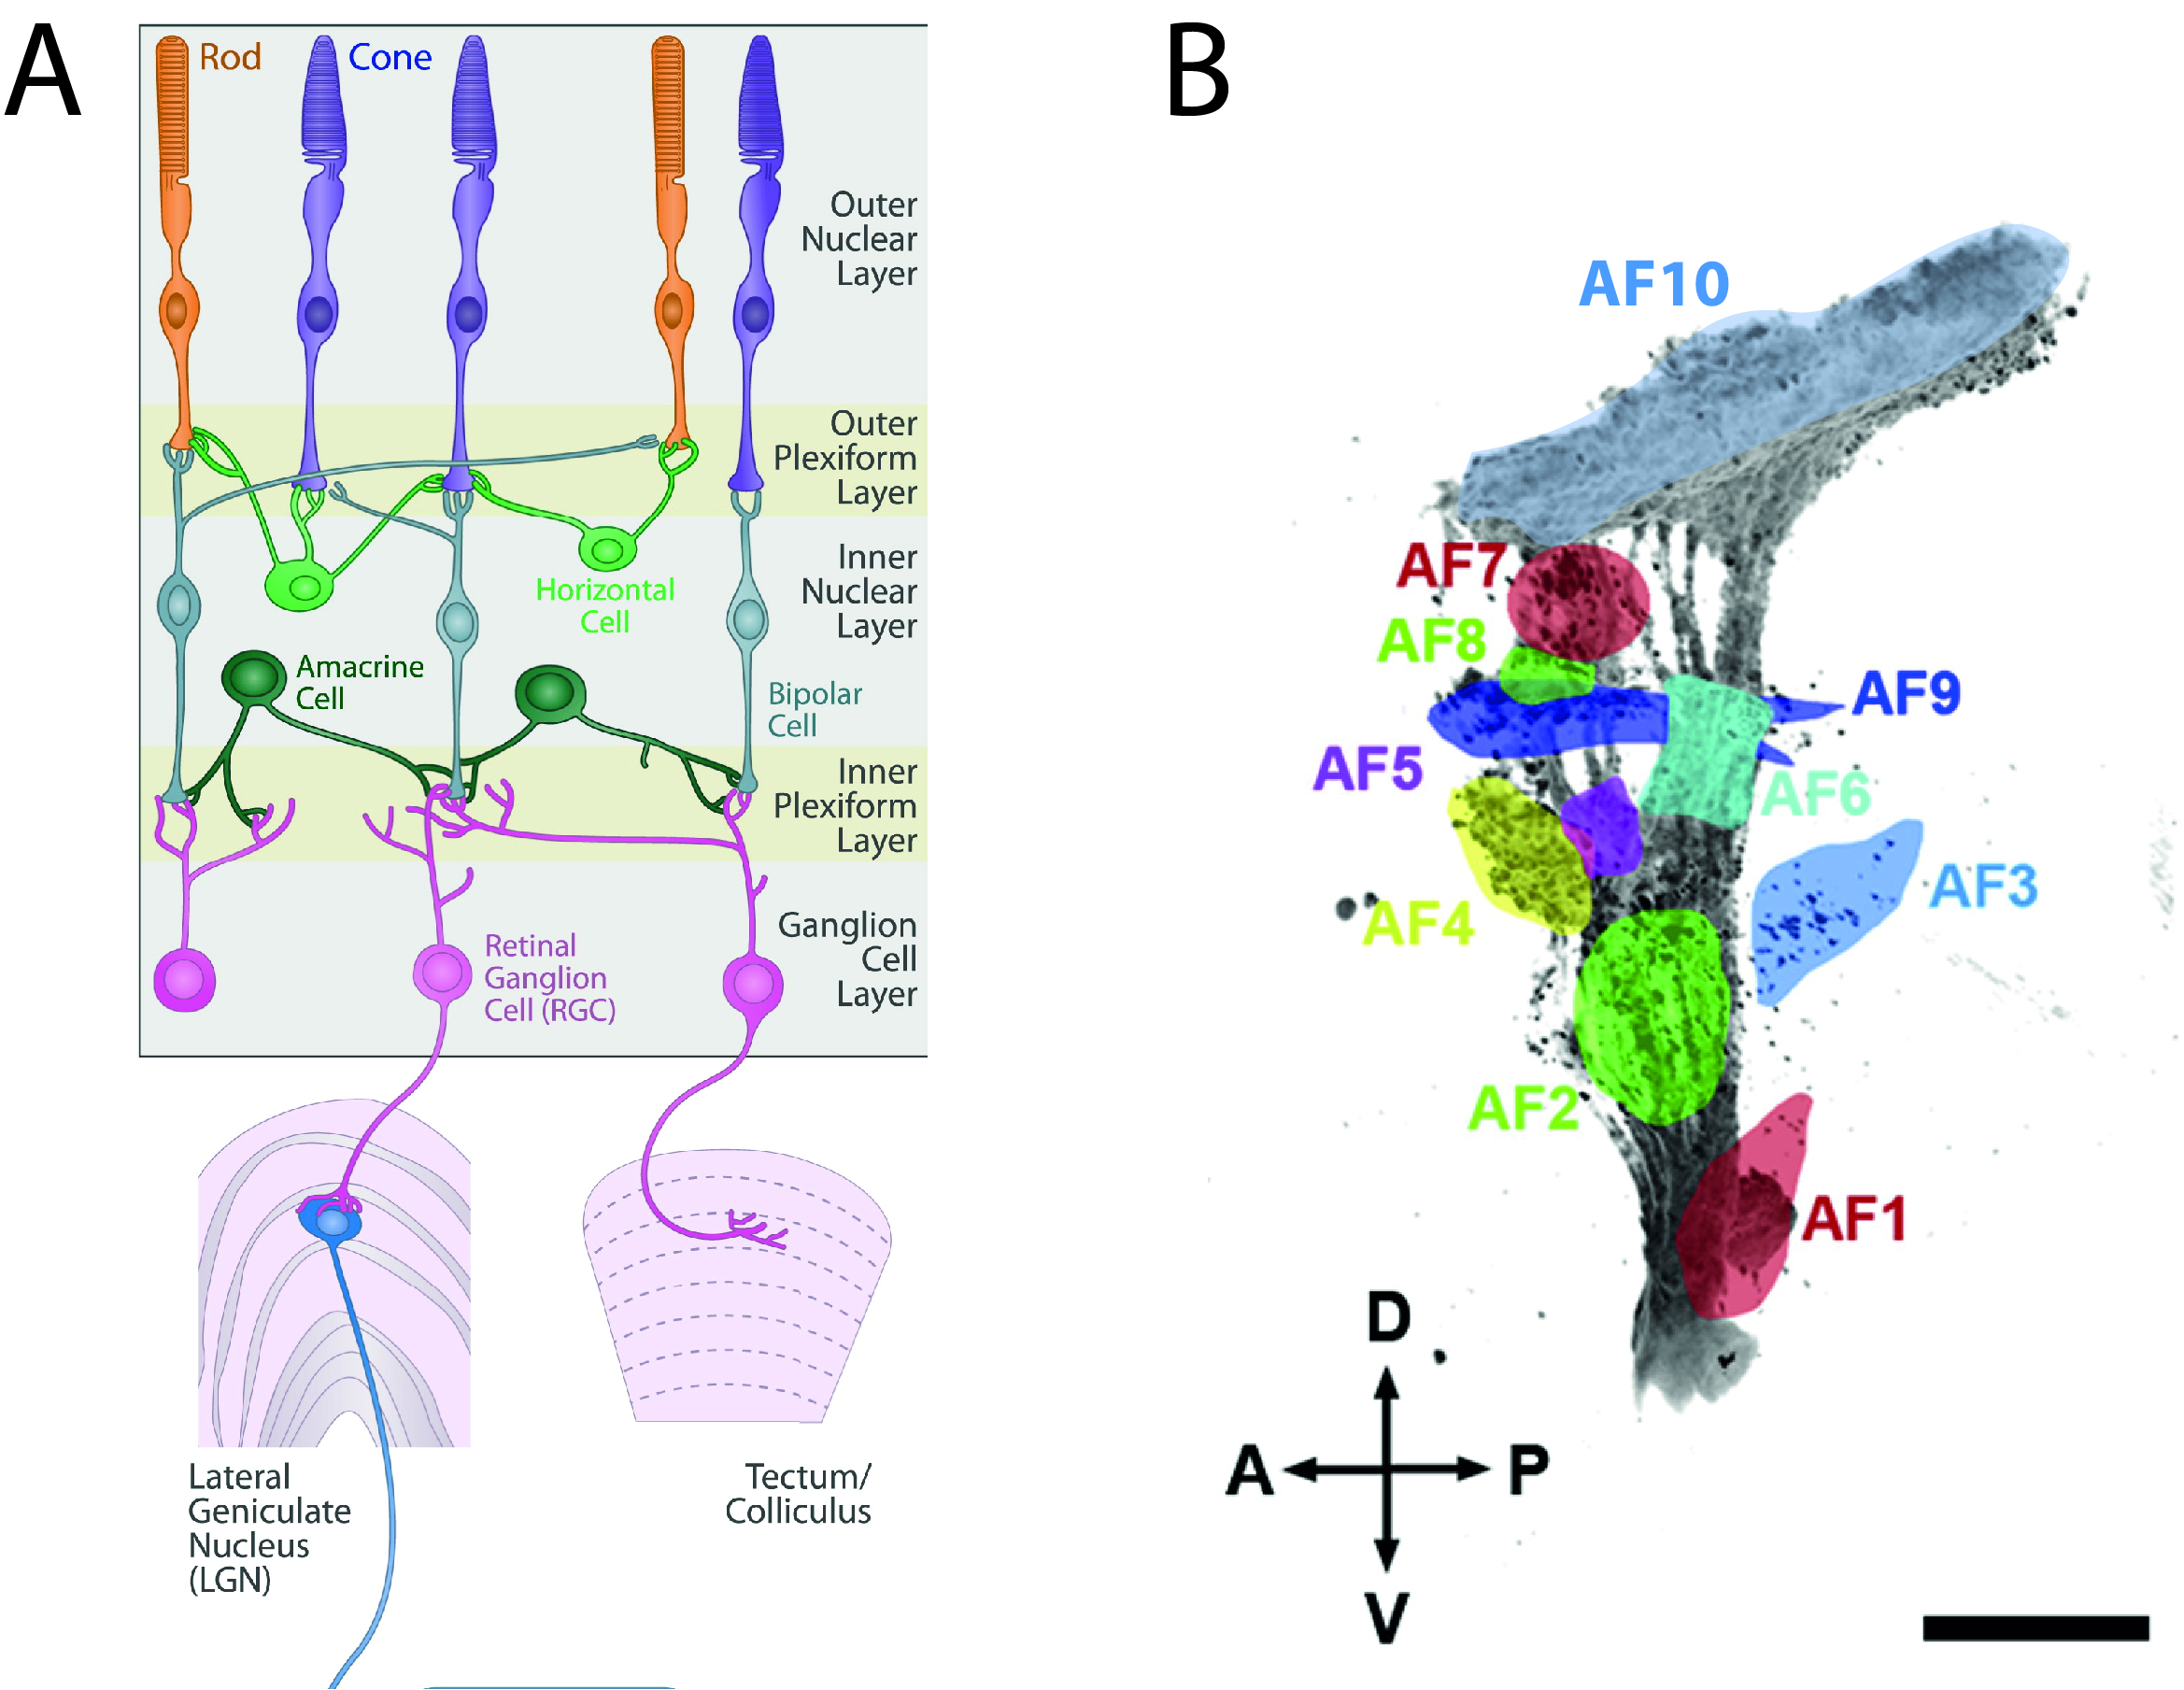
\includegraphics[width =  0.7\paperwidth]{Figures/retina_schematic.jpg}}
            \caption[\textbf{\label{fig:i_ret}\textbf{Cellular organisation of the retina and its targets.}}]{ \textbf{\label{fig:i_ret} Cellular organisation of the retina and its targets.} \textbf{(A)}  A schematic of the vertebrate visual system showing the organisation of the retina. The names of cell types, cellular layers and synaptic layers are reported. RGCs project to multiple regions of the brain including the superior colliculus (called optic tectum in lower vertebrates). In mammals RGCs also project to the visual cortex via the LGN. Image is from (\cite{Sanes2010DesignSystems}). \textbf{(B)} A 3D reconstruction of RGCs (grey) targeting multiple retinorecipient recipient regions of the brain. In fish there are 10 RGC retinorecipient areas called abourisation fields (AF1-10), the optic tectum is AF 10. Each arborisation field receives unique combinations of RGC subtypes. Image is from (\cite{Robles2014}).}
      \end{figure}

\subsection{Molecular cues guide axons to their targets.}
For the visual system to perform its function RGCs first need to be guided to their target regions and find their synaptic targets. Then within those regions precise connectivity needs to be established creating neural circuits that are capable of generating visually guided behaviours. Such circuitry is shaped by a combination of intrinsic and extrinsic factors.

In early visual system development, the axons of RGCs leave the retina, bundle together in the optic tract, and target retinorecipient regions of the brain. For many retinorecipient areas, this targeting of axons occurs in a manner that maintains the relative positions of the RGC somata in the retina, preserving a map of visual space in the target region (\cite{Luo2007DevelopmentMaps., Huberman2008MechanismsFields}). Such retinotopic maps are widespread in the visual system but perhaps one of the best studied is that of the optic tectum (\cite{Goodhill2005}). In fish and frogs, developing RGC axons exiting the eye fully decussate, targeting the contralateral tectum.  Axons originating in the nasal retina project to the anterior tectum and those stemming from the temporal retina terminate in the posterior tectum (\cite{Attardi1963PreferentialFibers}). Similarly, the dorso-ventral axis of the retina is transformed along the medio-lateral axis of the tectum. This preservation of the visual map in tectal coordinates requires relatively precise targeting of axons guided by molecular cues. The first evidence for this came from an elegant experiment by Sperry (\citeyear{Sperry1963CHEMOAFFINITYPATTERNS}) who was studying the regenerating retino-tectal pathway of frogs. In these experiments, the optic nerve was sectioned, the eye was rotated 180 degrees, and reattached so that the axons could regenerate. Sperry found that, despite this perturbation, regenerating RGC axons grew back to the same termination site, maintaining the same topographic order that they had previously held. This resulted in a reversed map of visual space and caused the frogs behaviour to be directed in the opposite direction to visual stimuli (\cite{Sperry1943EffectCoordination, Sperry1963CHEMOAFFINITYPATTERNS}) (\textbf{Figure \ref{fig:I_frog_sperry}}). This prompted the “chemoaffinity” hypothesis, in which the molecular tagging of axons and their targets acts as  “postal code”, guiding them to their termination site (Sperry 1963). Under this model, growing axon could be extended, retracted, or turned by regions of the target tissue expressing either attractive or repulsive cues (\cite{Meyer1998RogerHypothesis}). Further evidence for this model came from growing chick RGCs over stripes of tectal tissue in \textit{ex vivo} preparations. These demonstrated that RGCs from the temporal retina were repelled by stripes of posterior tectum and that this effect could be abolished through high temperature treatments that denatured proteins in the tectal substrate (\cite{Walter1987RecognitionVitro}).

\begin{figure}[!ht]
        \center{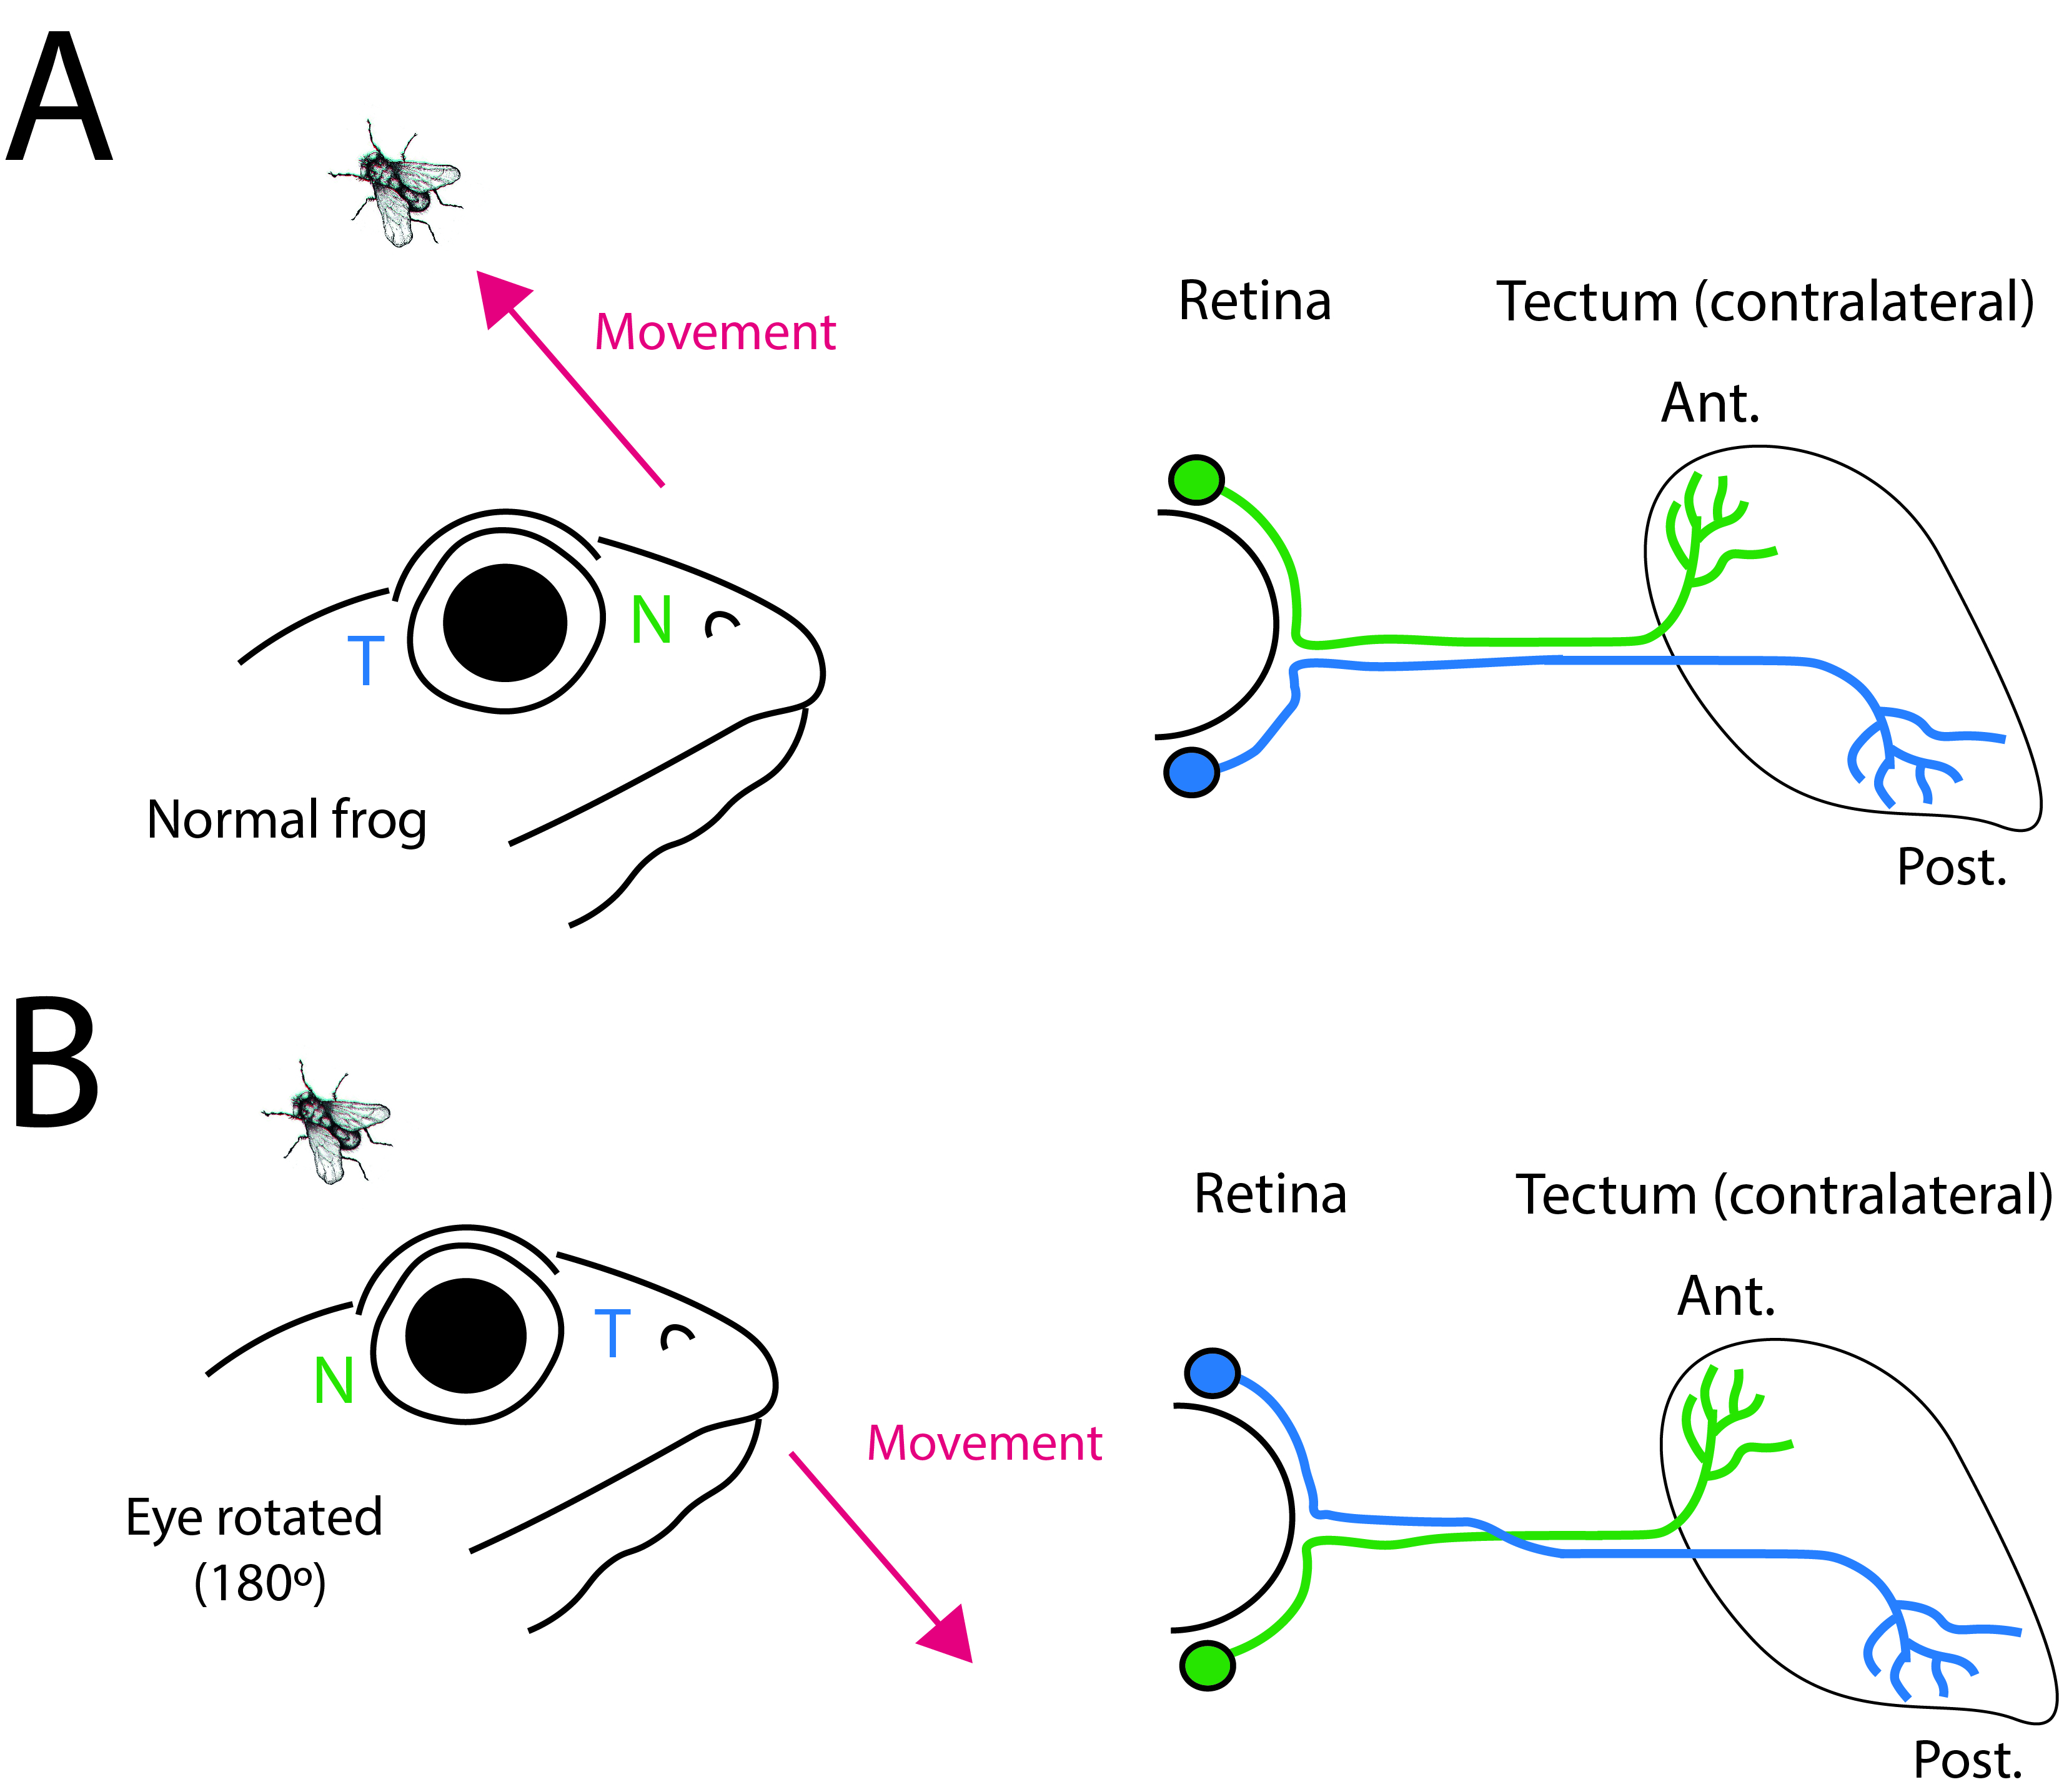
\includegraphics[width =  0.7\paperwidth]{Figures/I_frog_sperry.jpg}}
            \caption[\textbf{\label{fig:I_frog_sperry}\textbf{Sperry’s chemoaffinity hypothesis.}}]{\textbf{\label{fig:I_frog_sperry}Sperry’s chemoaffinity hypothesis.} Frogs are able to direct their behaviour towards their prey. RGCs positioned in the nasal retinal target anterior tectum (Ant.) whereas those with their somatas in temporal retina target the posterior tectum (Post.). Rotating the frog’s eye 180 degrees causes them to move in the opposite direction relative to visual stimuli. This is because the regenerating RGCs grow back to their original position within the tectum, resulting in a reversed map of visual space. For clarity the dorsal ventral axis have not been shown but these are also reversed.}
      \end{figure}

It is now known that numerous molecular cues are expressed within both the retina and tectum in complementary gradients. These exert a combined influence in positioning axon terminals within the tectum and many cues are well conserved across species (\cite{McLaughlin2003RetinotopicDevelopment, Feldheim2010VisualCompetition., Higenell2012ExpressionLaevis}). A large number of these identified cues belong to the ephrin family (\cite{Egea2007BidirectionalGuidance, Drescher1997TheGuidance}). Ephrins are membrane bound ligands which are expressed as a gradient within the tectum whereas their binding partners, the Eph receptors, are expressed by RGCs in gradients across the retina. The most well studied members of this family are EphrinA-EphA interactions, which allow for the temporal-nasal axis of the retina to be mapped to the anterior-posterior axis of the tectum (\cite{Triplett2012EphMaps}). This is because Ephrin-A is expressed in decreasing concentrations from the posterior to the anterior tectum (\cite{Drescher1995InKinases, Brennan1997TwoZebrafish, Higenell2012ExpressionLaevis, McLaughlin2003RetinotopicDevelopment}). This gradient repels Eph-A expressing RGCs from temporal retina, shifting their termination zone anteriorly (\cite{Drescher1997TheGuidance}). Blocking this pathway either through EphA knockout or pharmacological inhibition results in a disordered retinotectal map with axons overshooting their typical termination site (\cite{Woo2009RetinotopicAdhesion, Sweeney2015Ephrin-asTypes}). Similarly, the dorsoventral axis of the retina is thought to be mapped to the mediolateral tectum by EphB-EphrinB signalling and semaphorin3D, a molecule that repels ventral RGCs expressing neurophilin 1A/1D (\cite{Hindges2002EphBMapping., Brennan1997TwoZebrafish, Liu2012}). In addition to these, many more molecular cues have been identified in zebrafish through large scale mutagenesis followed by screening for retinotopic mapping defects (\cite{Baier1996GeneticProjection, Karlstrom1996ZebrafishPathfinding}). Together these studies show that numerous molecules are important for establishing retinotopic maps in the developing retinotectal system.

The action of molecular cues is not restricted to specifying retinotopy, and early work in chick showed that the laminar organisation of the tectum is also specified by molecular cues. For example, an extracellular protein, Nel, has been found to divert some RGC axons away from specific lamina (\cite{Jiang2009InNel}). In fish, a similar mechanism causes RGCs expressing the Robo2 receptor to target different regions of a superficial-to-deep gradient of Slit1 within the tectum (\cite{Xiao2011AssemblyCollagen}). This was thought to be significant because each of these lamina contain the terminal axons of RGCs that are tuned to stimuli moving in different directions. This suggests that molecular cues may be important for specifying cell-type-specific connections, potentially facilitating genetically predetermined tectal computations. However, this view was challenged by an experiment in a zebrafish line, known as the \textit{astray} mutant, which is a functional null for the Robo-2 receptor (\cite{Campbell2007Slit1aPathways}). While these mutants did show disorganised tectal lamina and deficits in the directional tuning of tectal neurons in early development, no functional deficits were found in later stages of development (\cite{Nikolaou2015LaminationCircuits}). This indicates that the establishment of lamina may be important for accelerating the development of tectal connections rather than cell-type-specific connectivity.

\subsection{Patterned activity propagates through the developing visual system}

Shortly after molecular cues direct developing RGCs to their targets, high levels of patterned neural activity can be found propagating throughout the developing visual system of many species (\cite{Pratt2016AnDevelopment}). There is a wealth of experimental evidence demonstrating that this activity plays a major role in shaping the organisation, connectivity, and physiological properties of sensory systems. A major source of this activity are retinal neurons responding to visual input. Naturalistic visual scenes contain changes in luminance and colour that are spatiotemporally structured. This spatial structure is reflected in the retina by causing neighboring neurons to be correlated in their firing (\cite{Demas2012VisionRetina}). Furthermore, as an organism moves through its environment the position of objects shift over the retina creating optic flow in the temporal to nasal direction, creating patterned activity structured in both space and time  (\cite{Hiramoto2014OpticInformation}). In species which develop externally, termed anamniotic, such as fish and frogs, visual experience can drive patterned activity throughout the visual system as soon as RGCs make their first synaptic connections with their projection targets (\cite{Holt1983OrderFibres}). Therefore visual experience is present at a time when neurons are establishing nascent connections, potentially shaping the refinement of this circuitry.

In contrast, amniotic species spend much of their development devoid of visual stimuli, either behind a thick shell, \textit{in ovo}, or within the womb, \textit{in utero} (\textbf{Figure \ref{fig:I_visual_expeirence_fig}}). Whilst visual stimulation has the potential to pattern the visual system post eye-opening or hatching, early visual system development must occur independently of such visually evoked activity. Nevertheless, in these species, it has been observed that there are high levels of  activity within the retina, which due to its apparent intrinsic generation is often called spontaneous activity. This activity takes the form of waves that travel over the retina and have been observed in multiple species including turtles (\cite{Sernagor1996InfluenceFields}), chicks (\cite{Wong1998DevelopmentallyRetina}), and various mammals (\cite{Meister1991SynchronousRetina, Wong1993TransientRetina, Torborg2005SpontaneousProjections, Ackman2012RetinalSystem, Warland2006DynamicsPathways}). In mammals, retinal waves occur in three stages: type I retinal waves that are driven by gap junctions, type II waves that are caused by starburst amacrine cells through the release of acetylcholine, and type III waves which require glutamate (\cite{Torborg2005SpontaneousProjections, Bansal2000MiceRetina, Kerschensteiner2016GlutamatergicWaves, Syed2004Stage-dependentRetina}). Early work on retinal waves relied on \textit{in vitro} preparations using retinal explants, revealing precise local correlations, reminiscent of those induced by visual stimulation  (\cite{Meister1991SynchronousRetina, Wong1993TransientRetina, Feller1996RequirementWaves}). In more recent work, Ackman et al., (2012) monitored neural activity in the terminals of RGCs in the SC of mice by bulk loading with a fluorescent reporter of activity and optically imaging the fluorescent changes. This revealed two things: firstly, that retinal waves propagate throughout the visual system and, secondly, that these waves are likely to move from temporal to nasal retina. The latter is particularly interesting because this travelling activation resembles activity that would be induced by optic flow in a swimming tadpole or fish, species in which retinal waves are either totally or largely absent (\cite{Kutsarova2017RulesBrain}). This has led to the suggestion that retinal waves exist as an evolutionary adaptation, compensating for the loss of visually evoked activity, made necessary by the transition of amniotic species to land and internal development (\cite{Pratt2016AnDevelopment}). 

Interestingly, despite developing externally, a single type of retinal wave has been identified in zebrafish (\cite{Zhang2016StereotypedAutoreceptors}). These occur very early in development, at a time-point when RGCs are making their initial synapses with tectal neurons, starting around 2.5 \gls{dpf} and finishing around 3 dpf. It is thought that retinal waves in fish may aid visual experience in shaping initial retinotectal connectivity, contributing to their relatively rapid visual system development. 

The literature on the role of activity, whether visually induced or intrinsic, in shaping the visual system is extensive. The following sections will highlight some of the classical experiments which have contributed to our understanding of this process. Particular focus will be devoted to the role of visual experience in shaping sensory maps, neuron morphology, and the functional properties of neurons within the visual system.




\begin{figure}[!ht]
        \center{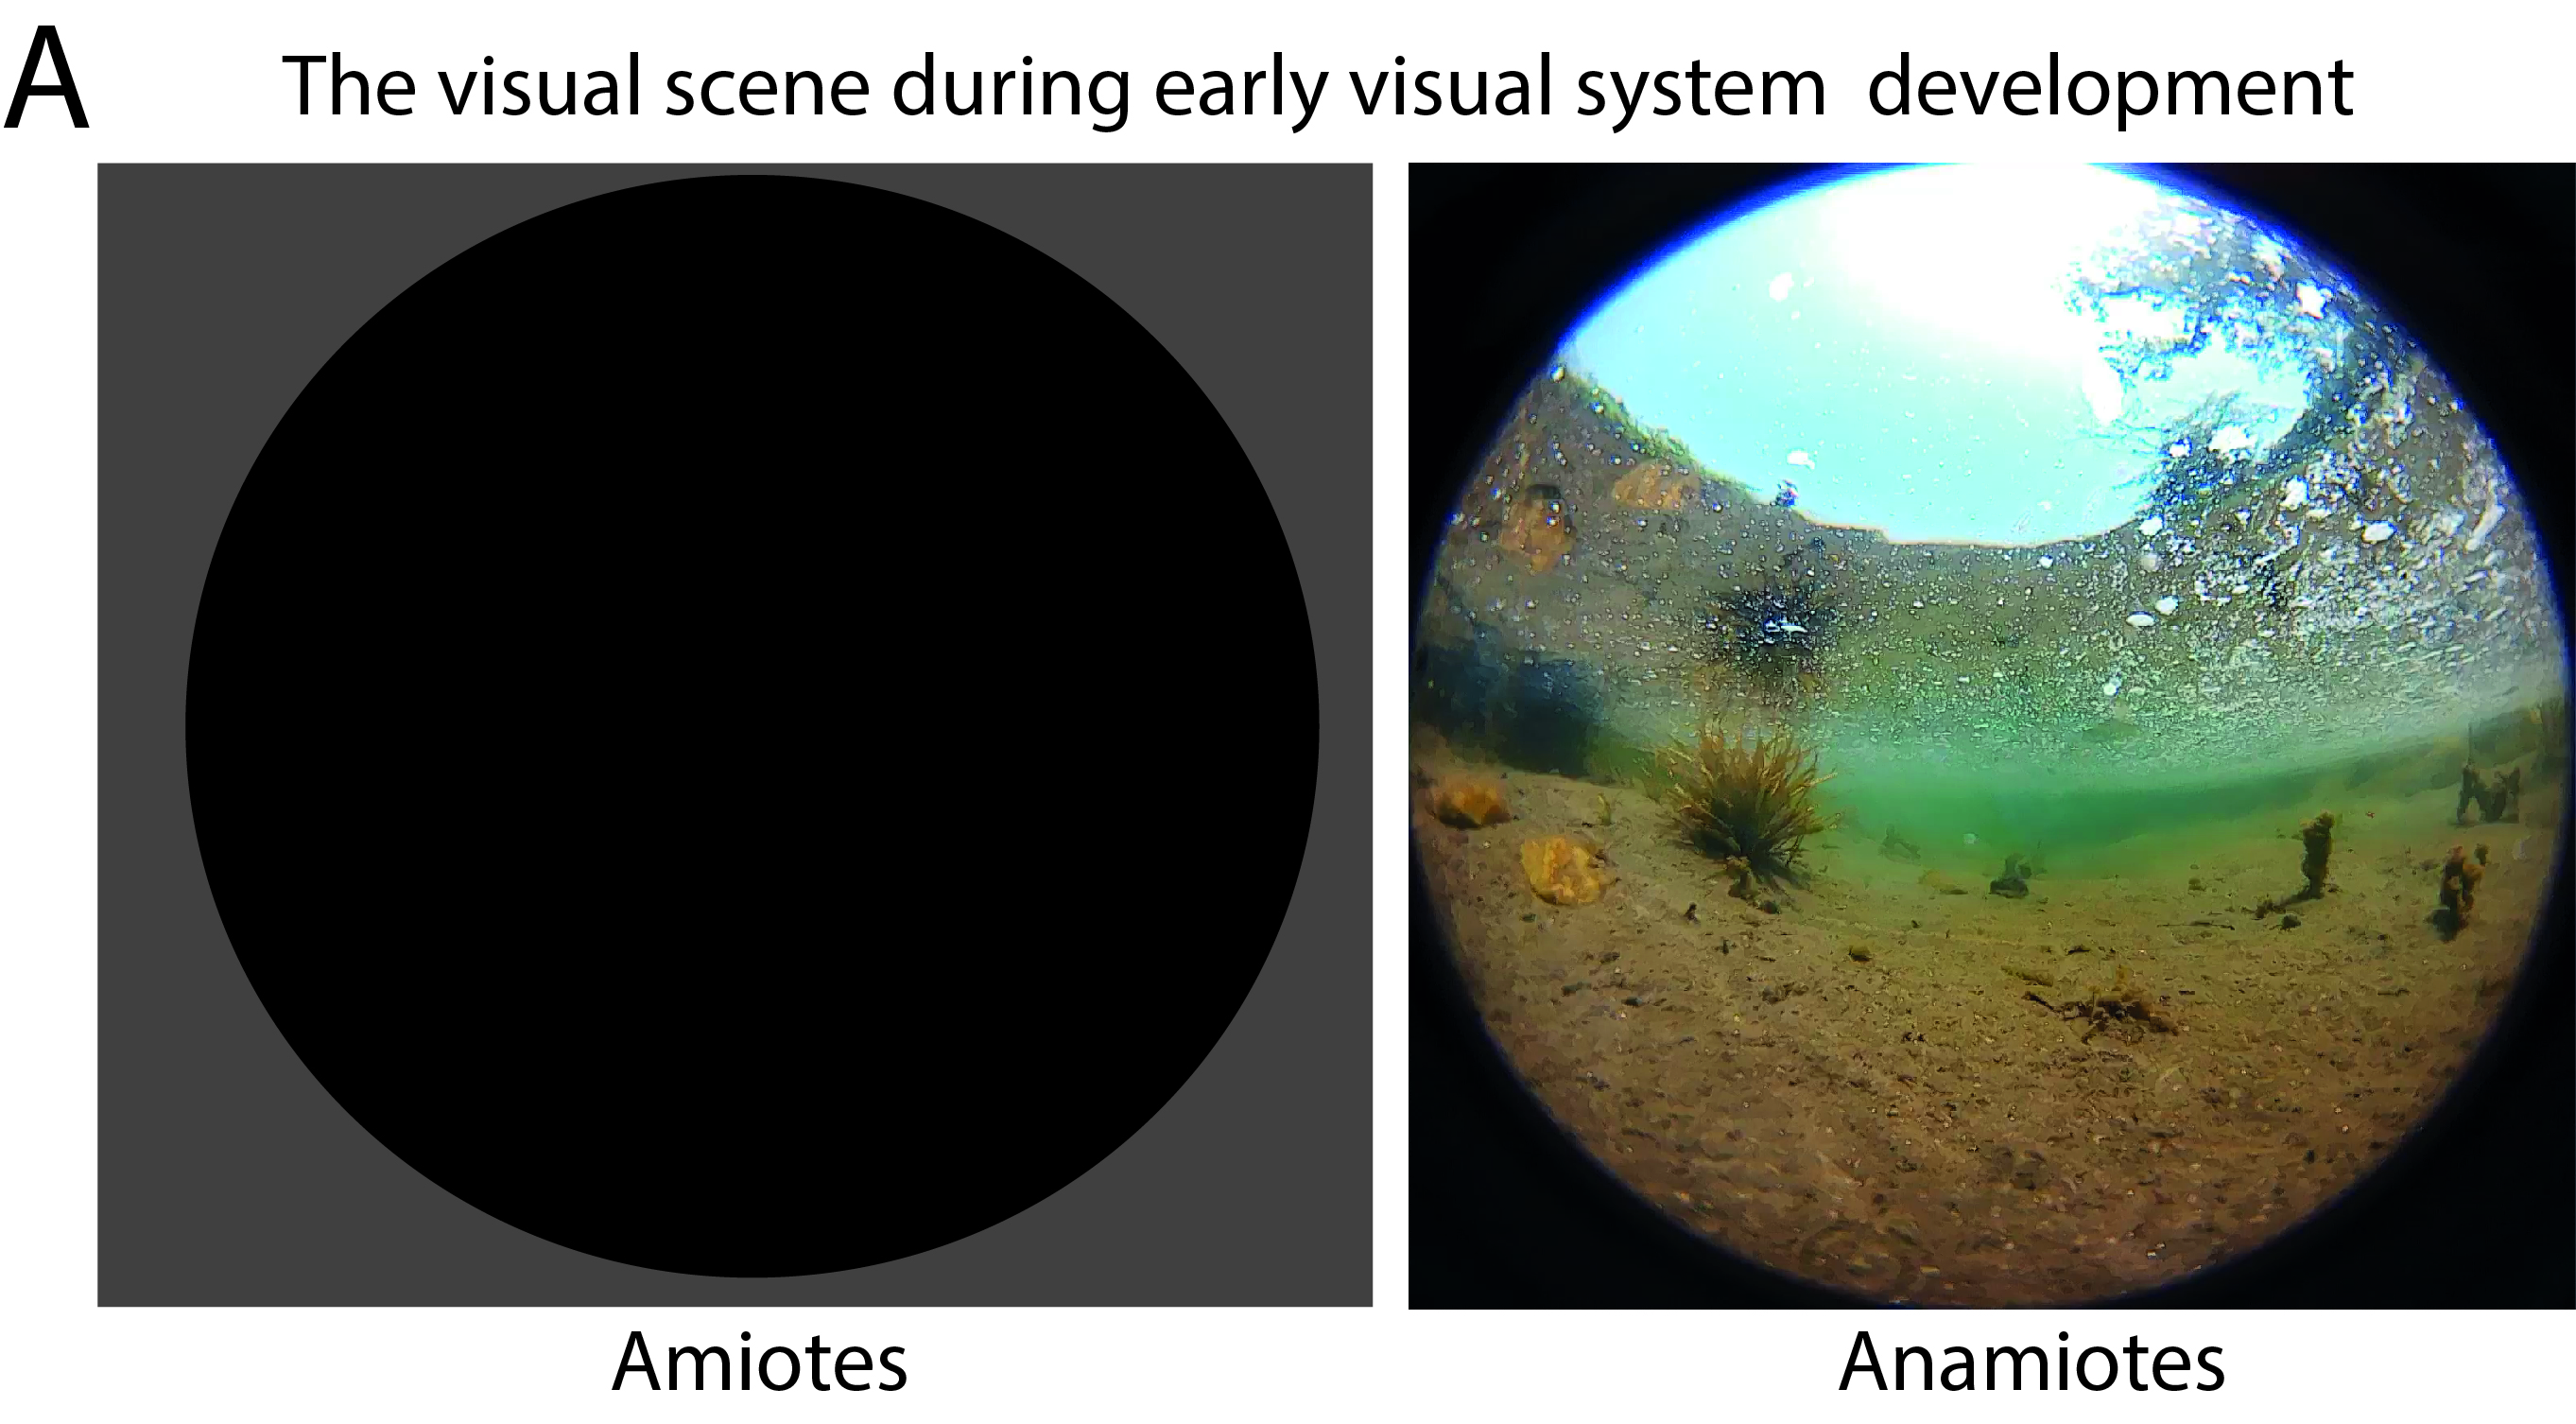
\includegraphics[width =  0.7\paperwidth]{Figures/I_visual_expeirence_fig.jpg}}
            \caption[\textbf{\label{fig:I_visual_expeirence_fig}\textbf{The extent of visual experience during early visual system development.}}]{ \textbf{\label{fig:I_visual_expeirence_fig}  The extent of visual experience during early visual system development.} \textbf{Left:} Amniotic species during early development are shielded from the visual world by their internal development, viewing total darkness (represented by the black circle). Therefore as neurons in the visual system are making their first synaptic connections they cannot be influenced by the visual environment. Instead they rely on spontaneously driven retinal waves to pattern the visual system. \textbf{Right:} An underwater photo of a natural zebrafish habitat.  As the development of anamniotic embryos takes place externally, they are exposed to visual scenes like this one as neural circuitry is forming. This visual stimulation activates RGCs and thier activity can be used to shape the visual system through activity dependent mechanisms. (Photo courtesy of Tom Baden)}

      \end{figure}

\subsection{Activity shapes the formation of visual maps}
\subsubsection{The formation of ocular dominance columns}
In mammals, outgrowing retinal projections do not fully decussate. Instead, a proportion of RGCs project ipsilaterally with the proportion of ipsilateral projections depending on the species (\cite{Larsson2011BinocularCoordination}). This means the SC, LGN, and visual cortex contain information originating from both eyes which may be important for generating binocular vision. In the cortex, this information is segregated into cortical bands known as \gls{od} columns (\cite{Hubel1969AnatomicalCortex}). Within these columns, cortical neurons show a preference in their responses to stimuli presented to either eye (\cite{Hubel1962ReceptiveCortex}). In a series of experiments, Hubel (\citeyear{Hubel1982Exploration1955-78}) and Wiesel (\citeyear{Wiesel1982PostnatalEnvironment}) showed that the development of this preference was highly dependent on visual experience. In these studies, an eye of a kitten or primate was sutured shut, depriving the eye of visual input (monocular deprivation - \acrshort{md}), and the animal was left to mature to adulthood. Removing the deprivation and performing electrophysiological recordings from single cortical neurons revealed that very few responses could be elicited when visual stimulation was given to the previously deprived eye. Instead, neurons showed a shift in responses towards the open eye, known as an OD shift (\cite{Hubel1970TheKittens, Hubel1977PlasticityCortex., Wiesel1963Single-cellEye, Wiesel1965ComparisonKittens.}). Furthermore, the effects of MD were found to be most pronounced within a particular developmental window in early development because MD outside of this window has little effect in shifting OD.  This suggested that the formation of OD columns could be altered by the lack of visual input, within a defined developmental period, known as the “critical period”, where the brain is in a highly plastic state (\cite{Hubel1970TheKittens}). 

In a second set of experiments Hubel and Wiesel demonstrated that the structure of OD columns were also affected by injecting radiolabeled amino acids into either  eye  in monkeys. This tracer was taken up by the RGCs projecting to the LGN where it transynapsaptically labelled thalamocortical projection neurons. This allowed for their axon terminals to be visualised within the visual cortex. Imaging sections of the visual cortex for autoradiography allowed for visualisation of OD columns as labelled and unlabeled bands (\textbf{Figure \ref{fig:I_sensory_maps}A}). In a monkey whose visual input has not been altered, these bands are of equal sizes, indicating that both eyes are equally represented within the cortex (\cite{Wiesel1974AutoradiographicTransport}). However, MD during development resulted in shrinkage of the OD bands representing the deprived eye (\cite{Hubel1977PlasticityCortex.}). This demonstrated that OD shifts were caused by gross anatomical changes in the regions of the cortex devoted to each eye. Together these observations indicate that there is a competitive mechanism between neurons based on activity, leading to more active afferents expanding their territory, forming more connections with cortical neurons at the expense of less active cells.

\begin{figure}[!ht]
        \center{\includegraphics[width =  0.7\paperwidth]{Figures/I_sensory_maps.jpg}}
            \caption[\textbf{\label{fig:I_sensory_maps}\textbf{Sensory maps can be reordered by changing activity patterns.}}]{ \textbf{\label{fig:I_sensory_maps} Sensory maps can be reordered by changing activity patterns.}  \textbf{(A)} Ocular dominance columns in layer 4 V1 of a normal macaque (\textbf{Top}) and in an animal that has undergone MD (\textbf{Bottom}). These were labelled by injecting a radiotracer into the eye with bands corresponding to the labeled eye in white. In the normal animal bands corresponding to either eye are equally sized. In the deprived animal the bands corresponding to the non-deprived eye (white) are expanded, occupying territory that would usually be occupied by the deprived eye (Top: \cite{Hubel1977PlasticityCortex.}, Bottom: LeVay et al., 1980). \textbf{(B)} Top: A three eyed frog, generated by transplanting one supernumerary eye during embryonic stages (\cite{Constantine-Paton1978Eye-specificFrogs}). This results in dual innervation of optic tectum. Middle: In a normal frog injecting a tracer labels into the eye labels only the contralateral tectal hemisphere (black). Bottom: In the three eyed frog injecting the radio tracer into the eye whose RGCs project to the same hemisphere as the supernumerary eye results in segregation of the input from the two eyes.  (\cite{Maya-Vetencourt2013Experience-DependentSystem}).
}
      \end{figure}

\subsubsection{Refinement of retinotopic maps in the optic tectum/SC}

 Early evidence seemed to suggest that activity is dispensable for the initial formation of retinotopic maps in the optic tectum. For example, blocking action potentials in the RGCs by injecting sodium channel blockers, such as \gls{ttx}, into the eye does not affect mapping between retina and tectum, as coarse retinotopic maps still form (\cite{Kobayashi1990DisturbanceGrayanotoxin, Meyer1983TetrodotoxinGoldfish, Olson1991TheProjection}). Additionally, in an imaginative experiment, Bill Harris transplanted an eye from an Axolotl into a \textit{Taricha torosa} newt (\cite{Harris1980TheSalamanders}). This species of newt naturally produces TTX but its neurons are unaffected by the toxin, meaning that only action potentials in the regenerating retinal projections were blocked. Despite the lack of activity in the retina, these projections still formed a crude retinotopic map within the newt tectum. This demonstrates that the initial establishment of retinotopic maps is activity-independent and is driven entirely by molecular cues.

Despite this, the initial topographic map is relatively coarse and has been shown to refine throughout development (\cite{Gaze1974TheXenopus}). More detailed experiments looking at point-to-point mappings within the tectum suggest that refinement is driven activity (\cite{Ruthazer2004InsightsPerspective}). For example, focal injections of neuronal tracers into the eye allow for a small number of developing or regenerating RGCs to be labelled and the area occupied by their terminals to be visualised in the tectum.  For similar sized focal injections into eyes where activity has been blocked by TTX, the area occupied by RGC terminals in the tectum is expanded (\cite{Kobayashi1990DisturbanceGrayanotoxin, Olson1991TheProjection},). Furthermore, this correlates with an expansion of the receptive field sizes on tectal neurons suggesting that the retinotopic map is less precise (\cite{Schmidt1983ActivityGoldfish}).

Some of the strongest early evidence for activity refining retinotectal maps comes from a study in which a third eye was grafted onto developing tadpoles (\cite{Constantine-Paton1978Eye-specificFrogs}). This caused a single tectal hemisphere, which usually exclusively receives projections from the contralateral eye, to be dually innervated by both the existing eye and the transplanted eye. If molecular cues were the only organising mechanism at play, then both eyes, expressing similar guidance cues, should display overlapping retinotopic maps that can be superimposed onto one another. In contrast to this, both eyes appear to segregate into eye specific stripes throughout the tectum, reminiscent of OD columns in the visual cortex (\cite{Law1981AnatomyTecta}) (\textbf{Figure \ref{fig:I_sensory_maps}B}). Similar results can also be produced by other manipulations that reroute retinal projections from the from the eye to the ipsilateral tectal hemisphere (\cite{Straznicky1979AnomalousAblation, Law1980RightAblations}). This indicates that, as the eyes are molecularly indistinguishable from one another, it must be the differences in the patterns of activity between the two eyes that organizes them into the bands. This was further supported through the observation that TTX applications could stop the segregation of inputs and could destabilise existing bands, showing that activity is needed for both their formation and maintenance (\cite{Meyer1982TetrodotoxinGoldfish, Boss1984ActivityGoldfish}). Furthermore, similar effects to those seen with TTX can be produced by blocking N-methyl-D-aspartate glutmate receptors (\acrshort{nmda}) specifically within the tectum showing that it is not only activity but also activation of postsynaptic tectal neurons that is important for organising these inputs (\cite{Reh1985Eye-specificPipiens.}). This implies that activation of postsynaptic neurons can instruct presynaptic input, presumably through a retrograde signal (\cite{Ruthazer2004InsightsPerspective}).

These early experiments raise a fundamental  question, what types of activity are important for driving this refinement? A number of studies have attempted to specifically look at how visual experience contributes to retinotopic map formation. One way to test this is to examine how the retinotopic maps develop in the absence of visual input by rearing the animal in complete darkness. Dark reared goldfish have slightly enlarged tectal multi-unit receptive field sizes, indicative of a more imprecise topographic map (\cite{Schmidt1985StroboscopicGoldfish}). However, in \textit{xenopus} frogs, receptive field sizes of dark reared animals were similar to that of controls (\cite{Keating1986VisualLaevis}). Additionally, dually innervated tecta of zebrafish still produce eye segregated bands when dark reared (\cite{Ramdya2008EmergenceCircuit}). While this may, as a first pass, suggest that visual experience does not contribute to retinotopic map formation, other manipulations of the visual scene have been found to have a much larger impact. For example, stroboscopic rearing, where flashes of light create correlated patterns of activity across the visual field, has been used to look at developing and regenerating retinotopic maps in fish (\cite{Schmidt1993ActivitydrivenSharpening, Schmidt1985StroboscopicGoldfish}). In both cases this led to enlarged receptive fields of tectal neurons and enlarged RGC terminals that failed to refine, suggesting that visual experience plays an instructive role on retinotopic map formation. However, perhaps the most compelling demonstration that visual experience shapes the retinotopic map relied on the observation that as frogs and fish swim forward, optic flow would induce activity in the retina in the temporal to nasal directions (T to N) (H\cite{Hiramoto2014OpticInformation}). Exposure to T to N optic flow in young tadpoles when the retinotopic map is poorly defined, results in the development of precise topography whereas when it is in the opposite direction (N to T) the map is poorly organised. This indicates that it may be specific types of visual experience that are important for instructing the formation of retinotopic maps.

As mentioned above, dark rearing appears to have a limited effect on establishing retinotopy compared to other manipulations of the visual scene. A potential reason for this is that dark rearing does not eliminate spontaneous activity. In mammals, spontaneous retinal waves are propagated through RGC terminals to the SC where they are thought to refine the topographic map (\cite{Pratt2016AnDevelopment}). A large amount of evidence for this hypothesis has been generated using the Chrnb2 \gls{ko} mouse (\cite{Rossi2001RequirementSystem,McLaughlin2003RetinotopicDevelopment,Mrsic-Flogel2005AlteredWaves}). This mutant lacks a subunit of the nicotinic acetylcholine receptor, which is required for the generation of Type II cholinergic waves. Retinal waves in this mutant lack a defined wave front, are more infrequent, and are more spatially distributed appearing as “flashes” across the retina (\cite{Burbridge2014VisualReceptors}). As a consequence retinotopic maps in the SC of these mutants are disrupted alongside deficits in eye specific segregation of RGC axons in the SC (\cite{McLaughlin2003RetinotopicDevelopment, Rossi2001RequirementSystem,Mrsic-Flogel2005AlteredWaves}). The overall activity level within the retina can be restored through either optogenetic or pharmacological manipulations, which rescue the deficit in eye segregation but not retinotopy (\cite{Zhang2012, Burbridge2014VisualReceptors}). In contrast to this, the Rx-$\beta$2 \gls{cko} mouse has lower overall activity in the retina but retains high local correlations between RGCs (\cite{Xu2015SpatialFrequency}). This mutant has eye segregation defects but retinotopic maps in the SC are indistinguishable from those in \gls{wt} mice. Together these studies indicate that it is the local correlational structure of retinal waves, rather than overall activity levels, that are important for organising retinotopy in the SC. Based on this it is possible that spontaneous activity that is seen in the retina of fish may compensate for the lack of visual experience in dark reared animals, allowing for retinotopic maps to still be refined (\cite{Kutsarova2017RulesBrain}). Interestingly, although retinal waves are not usually observed in frogs, dark rearing can induce increased local correlations between neighboring RGCs (\cite{Demas2012VisionRetina}), suggesting that there may in fact be common evolutionary mechanisms for coping with the absence of patterned visual input during development (\cite{Pratt2016AnDevelopment}).

\subsection{Activity regulates neuronal morphology and growth.}
Many observations which have demonstrated that activity shapes sensory maps have relied on bulk labeling of neurons using fluorescent or radioactive tracers. These have allowed for gross anatomical changes in neuroanatomy to be observed (\cite{Berry2016Experience-DependentSystem}). However, underlying these large scale changes are more subtle rearrangements in both axonal and dendritic arbours, altering neuronal structure and their connectivity with their neighbours. In the case of OD, individual thalamocortical neurons can be labeled in order to understand the effect of MD on the structure of axon terminals. This revealed that, after brief MD, the axonal arbours of afferents from the deprived eye begin to shrink (\cite{Antonini1993RapidCortex}). With longer periods of MD, it is found that the afferents of the non-deprived eye expand their territories, accounting for the population scale changes in OD columns (\cite{Antonini1996PlasticityCat.}). This suggests that the level of activity of a neuron may regulate the size of its arbour. 

The level of activity has also been found to be important for regulating RGC arbor size in zebrafish by genetically altering the level of activity in developing RGCs. For example, in the \textit{macho} mutant line of zebrafish, developing RGCs exhibit reduced sodium currents between 4-6 days \gls{dpf}, a period during which the retinotopic map is undergoing refinement (\cite{Gnuegge2001AnalysisMap}). The consequential silencing of RGCs leads to more extensive terminal abours, suggesting that they fail to refine in an activity-dependent manner. Similarly, the \textit{blumekhol} mutant expresses a mutated form of a vesicular glutamate transporter (vglut2a) in RGCs (\cite{Smear2007VesicularZebrafish}). This reduces glutamatergic release from RGCs and results in a similar phenotype to the macho mutant with larger terminal RGC arbours. This further indicates that “cross-talk” between developing RGCs and tectal neurons through synaptic activity is likely to be important for organising these inputs.

More nuanced manipulations have suggested that it is not simply the activity of neurons that shapes their growth, but their activity relative to their neighbours through competitive interactions. This can be shown by genetically silencing the activity of single RGCs, in an otherwise intact tectum. In one study, single RGCs were either hyperpolarized through the overexpression of an inward rectifying potassium channel, Kir 2.1, or were synaptically silenced through the expression of a dominant negative form of vesicle associated membrane protein (\cite{Hua2005RegulationCompetition}). Both manipulations resulted in a reduction in axon motility, leading to reduced total arbour length and branching complexity. Interestingly, this phenotype can be rescued if activity in neighbouring neurons is also suppressed. This suggests that decreased neural activity relative to neighbouring neurons leads to restricted growth. However, a more recent study, which also silenced synaptic activity in single developing RGCs through the expression of exogenous tetanus toxin, found the opposite effect (\cite{Fredj2010SynapticProjection}). Rather than reducing in size, the developing arbours failed to arrest growth resulting in an increase in total arbour length, although this effect could also be rescued through the suppression of neighbouring neurons. One potential reason for this is that these studies utilise different genetic promoters, potentially labelling different RGC subtypes. This hypothesis suggests that activity plays different roles in modulating arbour extensions in different cell types. Alternatively, the degree of silencing by each of these manipulations may be differ ultimately leading to different effects on arbour length and branching complexity. Regardless, both studies restore the arbour size to that of controls by inhibiting neighbouring neurons (\cite{Kita2015TopographicZebrafish}). This reaffirms that it is the level of activity relative to its neighbours that is important for shaping arbour growth, through a competitive interaction between neurons. 

\subsubsection{Activity dependent synaptotropic growth}
Time-lapse imaging in fish and frogs allows for the structure of singly labelled RGC axons and tectal dendrites to be visualised as they are growing, allowing for detailed studies into how activity affects arbour growth (\cite{ORourke1990DynamicStudy, Kaethner1992DynamicsAxons}). This has demonstrated that developing arbours go through a rapid phase of growth within the first few days and followed by a plateau (\cite{Wu1999DendriticMaturation, Cline2001DendriticSynaptogenesis, Meyer2006EvidenceMechanisms, Niell2004InArbor}). Within the initial growth period, arbours are highly dynamic, extending and retracting motile small filopodia with only a small fraction of these arbours being retained and stabilized. Even once the growth plateaus, branches are still extended and retracted at a slower rate and receptive fields of tectal neurons continue to refine suggesting that synaptic inputs are still being remodelled (\cite{Zhang2011FunctionalZebrafish}). A number of studies have highlighted that axon and dendrite growth is regulated by the formation of synapses, through a process of synaptotropic growth (\cite{Niell2004InArbor, Ruthazer2006StabilizationMaturation, Meyer2006EvidenceMechanisms}). Under this process, developing arbors send out large numbers of filopodia,  sampling the surrounding area and making nascent synapses. Only those that make the correct contacts are maintained, forming more mature synapses, whereas incorrect contacts are eliminated. These newly matured synapses then serve as branch points for newly extending filopodia.  Synaptotropic  growth therefore allows a developing arbour to preferentially explore a region where there is more likely to be correct contacts (\cite{Cline2001DendriticSynaptogenesis}). 

The stabilization of “correct contacts” is thought to be driven by correlated visually evoked activity between neurons (\cite{Ruthazer2006StabilizationMaturation}) through the activation of the NMDAR (\cite{Ruthazer2003ControlVivo}), the only glutamatergic receptor present at early/nascent synapses. Consistent with this, imaging a single developing axon in tadpoles that have dually innervated tecta suggests this dynamic process of growth is modulated by correlated activity between neurons (\cite{Ruthazer2003ControlVivo}). Here, the developing RGCs extend their filopodia with equal probability in all directions but branches are eliminated at a higher rate in territories that are occupied by the opposite eye. This suggests that branches are preferentially stabilized in regions of higher correlation that are occupied by RGCs from the same eye, which underlies the formation of eye specific bands. This process relies on postsynaptic glutamate activity since  blocking NMDARs abolishes this preferential stabilisation. In addition, Munz et al., (2014) took advantage of stray ipsilateral retinotectal projections to look at the effects of synchronous vs asynchronous visual stimulation to each eye on arbour growth. Here, synchronous activity between the two eyes promoted synapse formation in the stray axon, leading to similarly sized arbours as those in the contralateral projection. Asynchronous stimulation, on the other hand, resulted in a rapid increase in both branch additions and eliminations. This occurred alongside a decreased synaptic drive onto tectal neurons, suggesting that synapses are not mature. This shows correlated activity is required for the maturation of synaptic contacts and for the stabilization of developing branches, an effect that can be mimicked by NMDAR blockage (\cite{Munz2014RapidStimulation}). Together these experiments suggest that growth is directed by synapse formation in regions of correlated visual activity, in a process that is NMDAR dependent.

As RGC arbours are elaborating so must the dendritic arbours of their postsynaptic partners. It is therefore not surprising that tectal dendrites are equally as dynamic during development and also display highly heterogeneous branching patterns. Throughout this growth, tectal neurons receive synaptic input from the retina, suggesting that synaptic activity may be able to modulate this growth process. Consistent with this, blocking glutamatergic activity using NMDAR antagonists stops dendritic growth in the early stages of tectal development (\cite{Rajan1998GlutamateVivo}). To understand if visual experience has a direct role in modulating the growth of dendritic arbours, tectal neurons were timelapse imaged in vivo following 4 hour periods of either total darkness or the exposure to a moving stimulus (\cite{Sin2002DendriteGTPases}).   Imaging the same neurons within both conditions allows for comparison of growth rates, which enables subtle changes in growth to be examined that would otherwise be missed when averaging across populations. This revealed that exposure to visual stimuli promotes dendritic arbour growth, whereas in periods of darkness arbour growth is slowed. Furthermore, this change in dendritic motility could be blocked via the application of NMDAR antagonists, showing that glutamatergic synaptic inputs regulate these  experience-dependent changes.  Therefore these experiments show that activity, and through visual experience in particular, is integral for shaping neurons morphology and growth. 


\subsection{Receptive field properties are shaped by activity}
\subsubsection{Orientation selectivity}
 By shaping the physical structure of neurons, activity serves to alter connectivity within the visual system. This changes the input onto neurons, which is important for shaping their receptive field properties. Throughout the visual pathway neurons have been found to be specifically tuned to the orientation of edges and lines (\cite{Hubel1968ReceptiveCortex, Passaglia2002, Niell2008HighlyCortex,Nikolaou2012ParametricTectum,Fisher2015OrientationDrosophila}). Although these orientation selective neurons are wide-spread among vertebrate species, their development has been most studied in the visual cortex of mammals. In carnivores specifically, orientation tuning is mapped across the cortex where neurons with similar orientation preferences are clustered together (\cite{Maldonado1997OrientationCortex}). Optical imaging in ferrets has shown that orientation bands are present two weeks prior to eye opening and adult-like levels of tuning are achieved one week after the eyes open (\cite{Chapman1999DevelopmentCortex}). Blocking retinal activity through TTX injections blocks the development of orientation selectivity in the cortex (\cite{Chapman1993DevelopmentDeprivation}). However, disentangling the role of visual experience and spontaneous activity is complicated by the fact that visual activity can be evoked through the eyelid, although the pattern of stimulation is distorted (\cite{Krug2001ResponsesLids, Spear1978StriateEyelids}). In light of this, animals have been dark reared prior to eye opening and orientation selectivity populations are still present, suggesting that spontaneous retinal activity is sufficient for initially establishing orientation selectivity (\cite{White2001TheCortex}). Consistent with this, artificially disrupting the structure of spontaneous activity by pharmacologically inhibiting ON-RGCs (\cite{Chapman2000CorticalActivity}) or stimulating the optic nerve (\cite{Weliky1997DisruptionActivity}) can drastically alter the emergence of orientation selectivity. After eye opening, dark rearing can inhibit the maturation of orientation selectivity in ferrets (\cite{White2001TheCortex}). However, double eye-lid suturing, which distorts the visual experience, results in a far more severe effect with orientation selectivity being nearly absent in this group (\cite{Chapman1993DevelopmentDeprivation, White2001TheCortex})(\textbf{Figure \ref{fig:I_OS_DS_f}A}). Together these experiments suggest that it is not the mere presence of visual experience that is important for the maturation of orientation selectivity, but the pattern that is caused by normal visual stimulation. 
 
In addition to the effects of sensory deprivation, a number of studies have investigated the plasticity of orientation selectivity in the cortex by stripe rearing, a procedure where animals are raised in visual environments containing contours of a single orientation. Typically this has been done by either rearing animals in striped cylinders or raising them wearing goggles that restrict the orientations that the animal is exposed too (\cite{Blakemore1970, Stryker1975ModificationReexamination, Freeman1973AlterationAsymmetries}). Electrophysiological studies in cats have led to mixed reports, with high variability in effects between studies and also between animals within the same study , potentially reflecting the sampling bias associated with single cell recordings (\cite{Blakemore1970, Stryker1975ModificationReexamination, Blakemore1977GeneticCortex.}). In contrast, optical imaging in ferrets shows low variability and demonstrates that, while all orientations are represented, there is a large over-representation for the experienced orientation (\cite{Sengpiel1999InfluenceCortex}). Similar effects of stripe rearing have also more recently been seen in the visual cortex of mice with single cell resolution optical imaging (\cite{Kreile2011AlteredCortex}). This shows that the responses of neurons can be shifted towards the experienced orientation, suggesting that visual experience can play an instructive role in shaping orientation selectivity. 

\subsubsection{Direction Selectivity}
Just as neurons exhibit orientation selectivity, a substantial proportion of cells within the visual system respond significantly more to stimuli moving in a particular direction than to motion in the opposite direction, known as direction selectivity. Unlike orientation selectivity, direction selective neurons are absent from the visual cortex of ferrets at the time of eye opening and emerge two weeks after eye opening. This development is completely driven by patterned visual experience, with dark reared ferrets lacking directional tuning in V1 (\cite{Li2006TheExperience})(\textbf{Figure \ref{fig:I_OS_DS_f}B}). Furthermore, briefly exposing these animals to stimuli moving in a single direction can induce tuning in that direction whilst leaving tuning for all other directions absent. Similar effects of experience on direction selectivity have been found in the optic tectum of \textit{xenopus} tadpoles. While direction selectivity is absent during the early developmental stages, exposing tadpoles to a bar that repeatedly travelled in a single direction can train neurons to respond selectivity to stimuli moving in that direction (\cite{Engert2002MovingNeurons}). This training can be abolished by the application of NMDA antagonists, indicating that it is mediated by synaptic glutamate activity. Together, these results show that visual motion in the environment can play an instructive, rather than permissive, role in the formation of direction selectivity.

Interestingly, this effect of visual experience may be species or brain region specific. This is because dark rearing zebrafish has no effect on the emergence of direction selectivity within RGCs or tectal neurons (\cite{Niell2005FunctionalTectum}; \cite{Ramdya2008EmergenceCircuit}; \cite{Lowe2013ADevelopment}). Similarly, direction selectivity in the superior colliculus of mammals can still emerge when animals are dark reared, although this tuning can be disrupted through strobe rearing (\cite{Chalupa1978DirectionalDark-rearing,Flandrin1975SuperiorKitten}). However, it is not known whether the sustained experience of a particular direction can alter these tuning profiles. 

Together the studies described so far show that many aspects of visual system development are genetically encoded, either through molecular cues specifying projection targets, or by spontaneous activity shaping neural circuits. However, extrinsic activity, driven by visual experience, has been shown to have profound effects on multiple aspects of visual system development including sensory maps, neuron morphology and the receptive field properties of neurons. This indicates that visual experience serves help mature neural circuits, or change their organisation all together. 



\begin{figure}[!ht]
        \center{\includegraphics[width =  0.6\paperwidth]{Figures/I_OS_DS_ferrret_2.jpg}}
            \caption[\textbf{\label{fig:I_OS_DS_f}\textbf{The effect of visual experience on the development of receptive field properties in the cortex. }}]{\textbf{\label{fig:I_OS_DS_f} The effect of visual experience on the development of receptive field properties in the cortex.} \textbf{(A)} Optical imaging of changes in the haemodynamic response in V1 to stimuli of different orientations in ferrets that have been normally reared (\textbf{left column}), dark reared (\textbf{middle column}) or lid sutured (\textbf{right column}). \textbf{Top row:} shows mean response to vertical stimuli. \textbf{Second row:}  the mean response to horizontal stimuli. textbf{third row:}  the difference between them. \textbf{Bottom row:} shows the maximum response to each orientation as color coded by legend. This shows that while orientation selectively is reduced in the dark reared group, it is almost absent in the lid sutured group. Thus, while visual experience is important for the maturation of orientation selectivity, abnormal patterns of visual stimulation can disrupt it. Images from (\cite{White2001TheCortex}). \textbf{(B)} Optic imaging of the haemodynamic response in V1 to stimuli moving in different directions in ferrets that have been normal reared (\textbf{left column}) or dark reared (\textbf{right column}). \textbf{Top row:} shows the mean response to stimuli moving at 42 degrees (0 degrees = horizontal moving rightward). \textbf{bottom row:} A map colored by max response to each direction. This demonstrates that direction selectively does not form in dark reared animals (\cite{Li2006TheExperience}). 

        }
      \end{figure}



\subsection{Hebbian plasticity and the NMDAR}
A core conceptual framework underlying many of the activity-dependent changes discussed above is that of Hebbian plasticity. Hebbian plasticity is the notion that correlated firing between pre- and postsynaptic neurons causes an increase in the synaptic efficacy between them  (long term potentiation - LTP) whereas decorrelated activity between neurons leads to decreased synaptic efficacy (long term depression - LTD) (\cite{Hebb1949, Stent1973ALearning.}) (\textbf{Figure \ref{fig:I_hebbian_plasiticty_fig}A}). Confirmation of Hebb’s rule in hippocampal cultures indicated that high frequency tetanic stimuli could induce LTP whereas low frequency stimulation resulted in LTD (\cite{Bliss1973LonglastingPath, Kemp2004HippocampalAccquisition,Dudek1992HomosynapticBlockade}). In addition to this, experiments in the optic tectum of frogs suggested that synaptic plasticity could be bidirectionally regulated by the relative timing of pre- and postsynaptic spikes (\cite{Zhang1998ASynapses}). In these experiments, tectal cells were patched alongside RGCs allowing for controlled stimulation of these neurons relative to each other. By shifting the relative timings between pre- and postsynaptic neurons, it was shown  that LTP could be induced if the RGC fired prior to the tectal neuron, whereas LTD was induced if this order is reversed. The extent of this synaptic modulation was found to be asymmetrically proportional to the time interval relative to the postsynaptic spike, exponentially decaying over a 10 msec time window,  a phenomenon known as \gls{stdp} (\cite{Mu2006SpikeSystem}) (\textbf{Figure \ref{fig:I_hebbian_plasiticty_fig}B}).  This gives a mechanism by which temporally organised spiking patterns can shape synaptic connectivity. Importantly, different visual scenes contain different statistics, producing unique spiking patterns. Therefore, Hebbian mechanisms potentially underlie the instructional influence that the visual environment exerts over the developing visual system. Consistent with this, LTP can be induced through visual stimulation (\cite{Zhang2000VisualSynapses}) and Hebbian plasticity has been implicated in numerous aspects of experience-dependent development in the visual system, including the formation of retinotopic maps (\cite{Ruthazer2003ControlVivo}), neuron growth (\cite{Munz2014RapidStimulation, Sin2002DendriteGTPases}), and direction selectivity (\cite{Engert2002MovingNeurons, Mu2006SpikeSystem}).

A critical component of the Hebbian framework is the NMDAR, an ion channel situated on the postsynaptic membrane that is usually occluded by a Mg2+ ion at rest. The channel requires both binding of glutamate released from the presynaptic neurons and depolarisation of the postsynaptic neuron to occur in order to relieve this block, allowing current to influx (\cite{Nowak1984MagnesiumNeurones}) (\textbf{Figure \ref{fig:I_hebbian_plasiticty_fig}C}). This property of the channel allows it to act as a molecular detector of correlated activity between pre- and postsynaptic activity (\cite{Yashiro2008RegulationMetaplasticity}). Notably, NMDAR antagonists have been shown to abolish LTP formation through STDP rules in vivo (\cite{Zhang1998ASynapses}). When the channel is activated, Ca2+ flows into the cell and triggers intracellular cascades that can lead to synaptic modification. It is thought that the amount of calcium influx is important for the direction of plasticity, with large calcium influx resulting in LTP and small influx causing LTD (\cite{Yashiro2008RegulationMetaplasticity}). In the developing brain, LTP leads to synapse maturation and stabilisation by activating \gls{camkii} which triggers an intracellular cascade.  This cascade causes glutamatergic channels \gls{ampa} receptors to the synaptic membrane,  potentiating subsequent synaptic currents (\cite{Wu1996MaturationSynapse,Wu1998StabilizationCaMKII,Rajan1998GlutamateVivo}). LTD, on the other hand, leads to a reduction in AMPA currents (\cite{Munz2014RapidStimulation}). This mechanism may therefore underlie the selective stabilization of axonal and dendritic branches in regions of correlated activity via synaptotropic growth. Over time, this stabilisation within coactive environments and elimination from non-correlated areas could refine retinotopic maps or eye-specific territories (\cite{Ruthazer2003ControlVivo, Munz2014RapidStimulation}). Consistent with this, NMDAR activity induced by visual experience can lead to modifications in cytoskeletal dynamics via GTPase activity, thereby altering neuron morphology (\cite{Sin2002DendriteGTPases}). Visual experience has also been found to increase glutamatergic synaptic strength by increasing its AMPA receptor contribution, or by shifting AMPA/NMDAR ratio at synapses (\cite{Engert2002MovingNeurons}). Furthermore, inhibiting AMPA trafficking has been shown to block experience-dependent dendritic arbour growth in tectal neurons (\cite{Haas2006AMPAVivo}). Therefore, Hebbian plasticity, facilitated by the NMDAR, gives a mechanism by which neural activity can shape neural connectivity in the developing brain.

\subsubsection{Synaptic plasticity is regulated by NMDAR subunit composition}

The amount of calcium that flows through the NMDAR, and therefore the direction of synaptic plasticity, is  dependent on the subunit composition of the NMDAR (\cite{Yashiro2008RegulationMetaplasticity}). NMDAR are heteromeric tetramers containing two obligatory NR1 subunits and two regulatory subunits that can be N2RA-D or NR3A-B (\cite{Cull-Candy2004RoleSynapses., Al-Hallaq2007NMDAHippocampus}). The majority of the NMDAR’s functional diversity comes from the NR2 subunits. Of these, NR2A and NR2B are most studied due to their elevated expression within the brain, and their differential current kinetics (\cite{Yashiro2008RegulationMetaplasticity}). NR2A-containing synapses have higher opening probability and faster deactivation than NR2B-containing synapses (\cite{Chen1999Subtype-dependenceProbability,Monyer1994DevelopmentalReceptors, Erreger2005Subunit-specificProfiles}). Despite this lower opening probability, the NR2B, due to its slow deactivation, carries around two-fold Ca2+ current through a longer current decay (\textbf{Figure \ref{fig:I_hebbian_plasiticty_fig}D}). Therefore, activation of these different receptors alters the amount of Ca2+ influx through the receptor pore, potentially modulating the direction of plasticity.  The precise relationship between NR2 subunits and the induction LTP/LTD remains controversial (\cite{Liu2004RolePlasticity, Massey2004DifferentialDepression}). However, it has been suggested that, while either subunit can facilitate both forms of plasticity, the NR2A/NR2B ratio at a synapse controls the threshold for synaptic plasticity, acting as a form of metaplasticity over synaptic plasticity (\cite{Philpot2007ObligatoryCortex,Yashiro2008RegulationMetaplasticity}). Under this hypothesis, NR2A dominated synapses are more likely to undergo LTD than those that are dominated by NR2B.

In the mammalian brain, the NR2A/NR2B ratio varies between brain regions and developmental stages (\cite{Cull-Candy2001NMDADisease}).  In the cortex, there is a developmental switch in which NR2B is expressed as the dominant subunit in the first postnatal week and NR2A expression increases shortly after (\cite{Monyer1994DevelopmentalReceptors};  \cite{Sans2000ASynapses, Sheng1994ChangingCortex}). Consistent with this expression pattern and the kinetics of the channels, NMDAR currents at cortical synapses have faster kinetics and a reduced sensitivity to NR2B selective channel blockers at later stages of development (\cite{Carmignoto1992Activity-dependentCortex, Flint1997, Tovar1999TheVitro}). The precise timing of this switch is thought to be regulated by neuronal activity and sensory experience. In dark reared animals, the expression of NR2A in the visual cortex is delayed but can be rapidly induced by just 1 hour exposure to visual experience (\cite{Quinlan1999BidirectionalDevelopment, Carmignoto1992Activity-dependentCortex,Quinlan1999RapidVivo,Philpot2001VisualCortex}).
This switch in NR2B/NR2A composition during development is thought to be crucial for mediating activity-dependent changes in the developing brain. Consistent with this, knocking out the NR2A subunit in mice can keep synapses in an immature state, retaining the longer NMDA currents of NR2B-containing synapses (\cite{Fagiolini2003SeparableSignaling}). In this mutant, the number of orientation selective neurons in the visual cortex is severely reduced. This may suggest that under normal conditions, the developmental switch shifts synapses towards LTD, refining the receptive field properties of neurons. Furthermore, genetic mutations in the \textit{Grin2a} gene, which encodes the NR2A subunit, have been associated with epilepsy in humans (\cite{Gao2017AAphasia}), Suggesting that correct NR2A function is important for shaping developing neural circuits in the brain.

The role of NMDA subunit composition in regulating the development of neural circuitry in non-mammalian vertebrates is virtually unknown, but the NR2A and NR2B subunits are extremely well conserved across species (\cite{Ewald2009CloningTadpoles}). The expression of NR2A is also found to lag behind that of the NR2B in zebrafish (\cite{White2017AZebrafish}). Knocking down the expression of the NR2A subunit in \textit{xenopus} tectal neurons reduces branch clusters, whereas knock down of the NR2B subunit has no effect (\cite{Ewald2008RolesVivo}). Therefore, it is possible that these subunits are important for shaping activity-dependent development of the visual system in different ways within these species. One of the aims of this thesis is to understand how this subunit composition facilitates experience-dependent in developing neural circuits.


\begin{figure}[!ht]
        \center{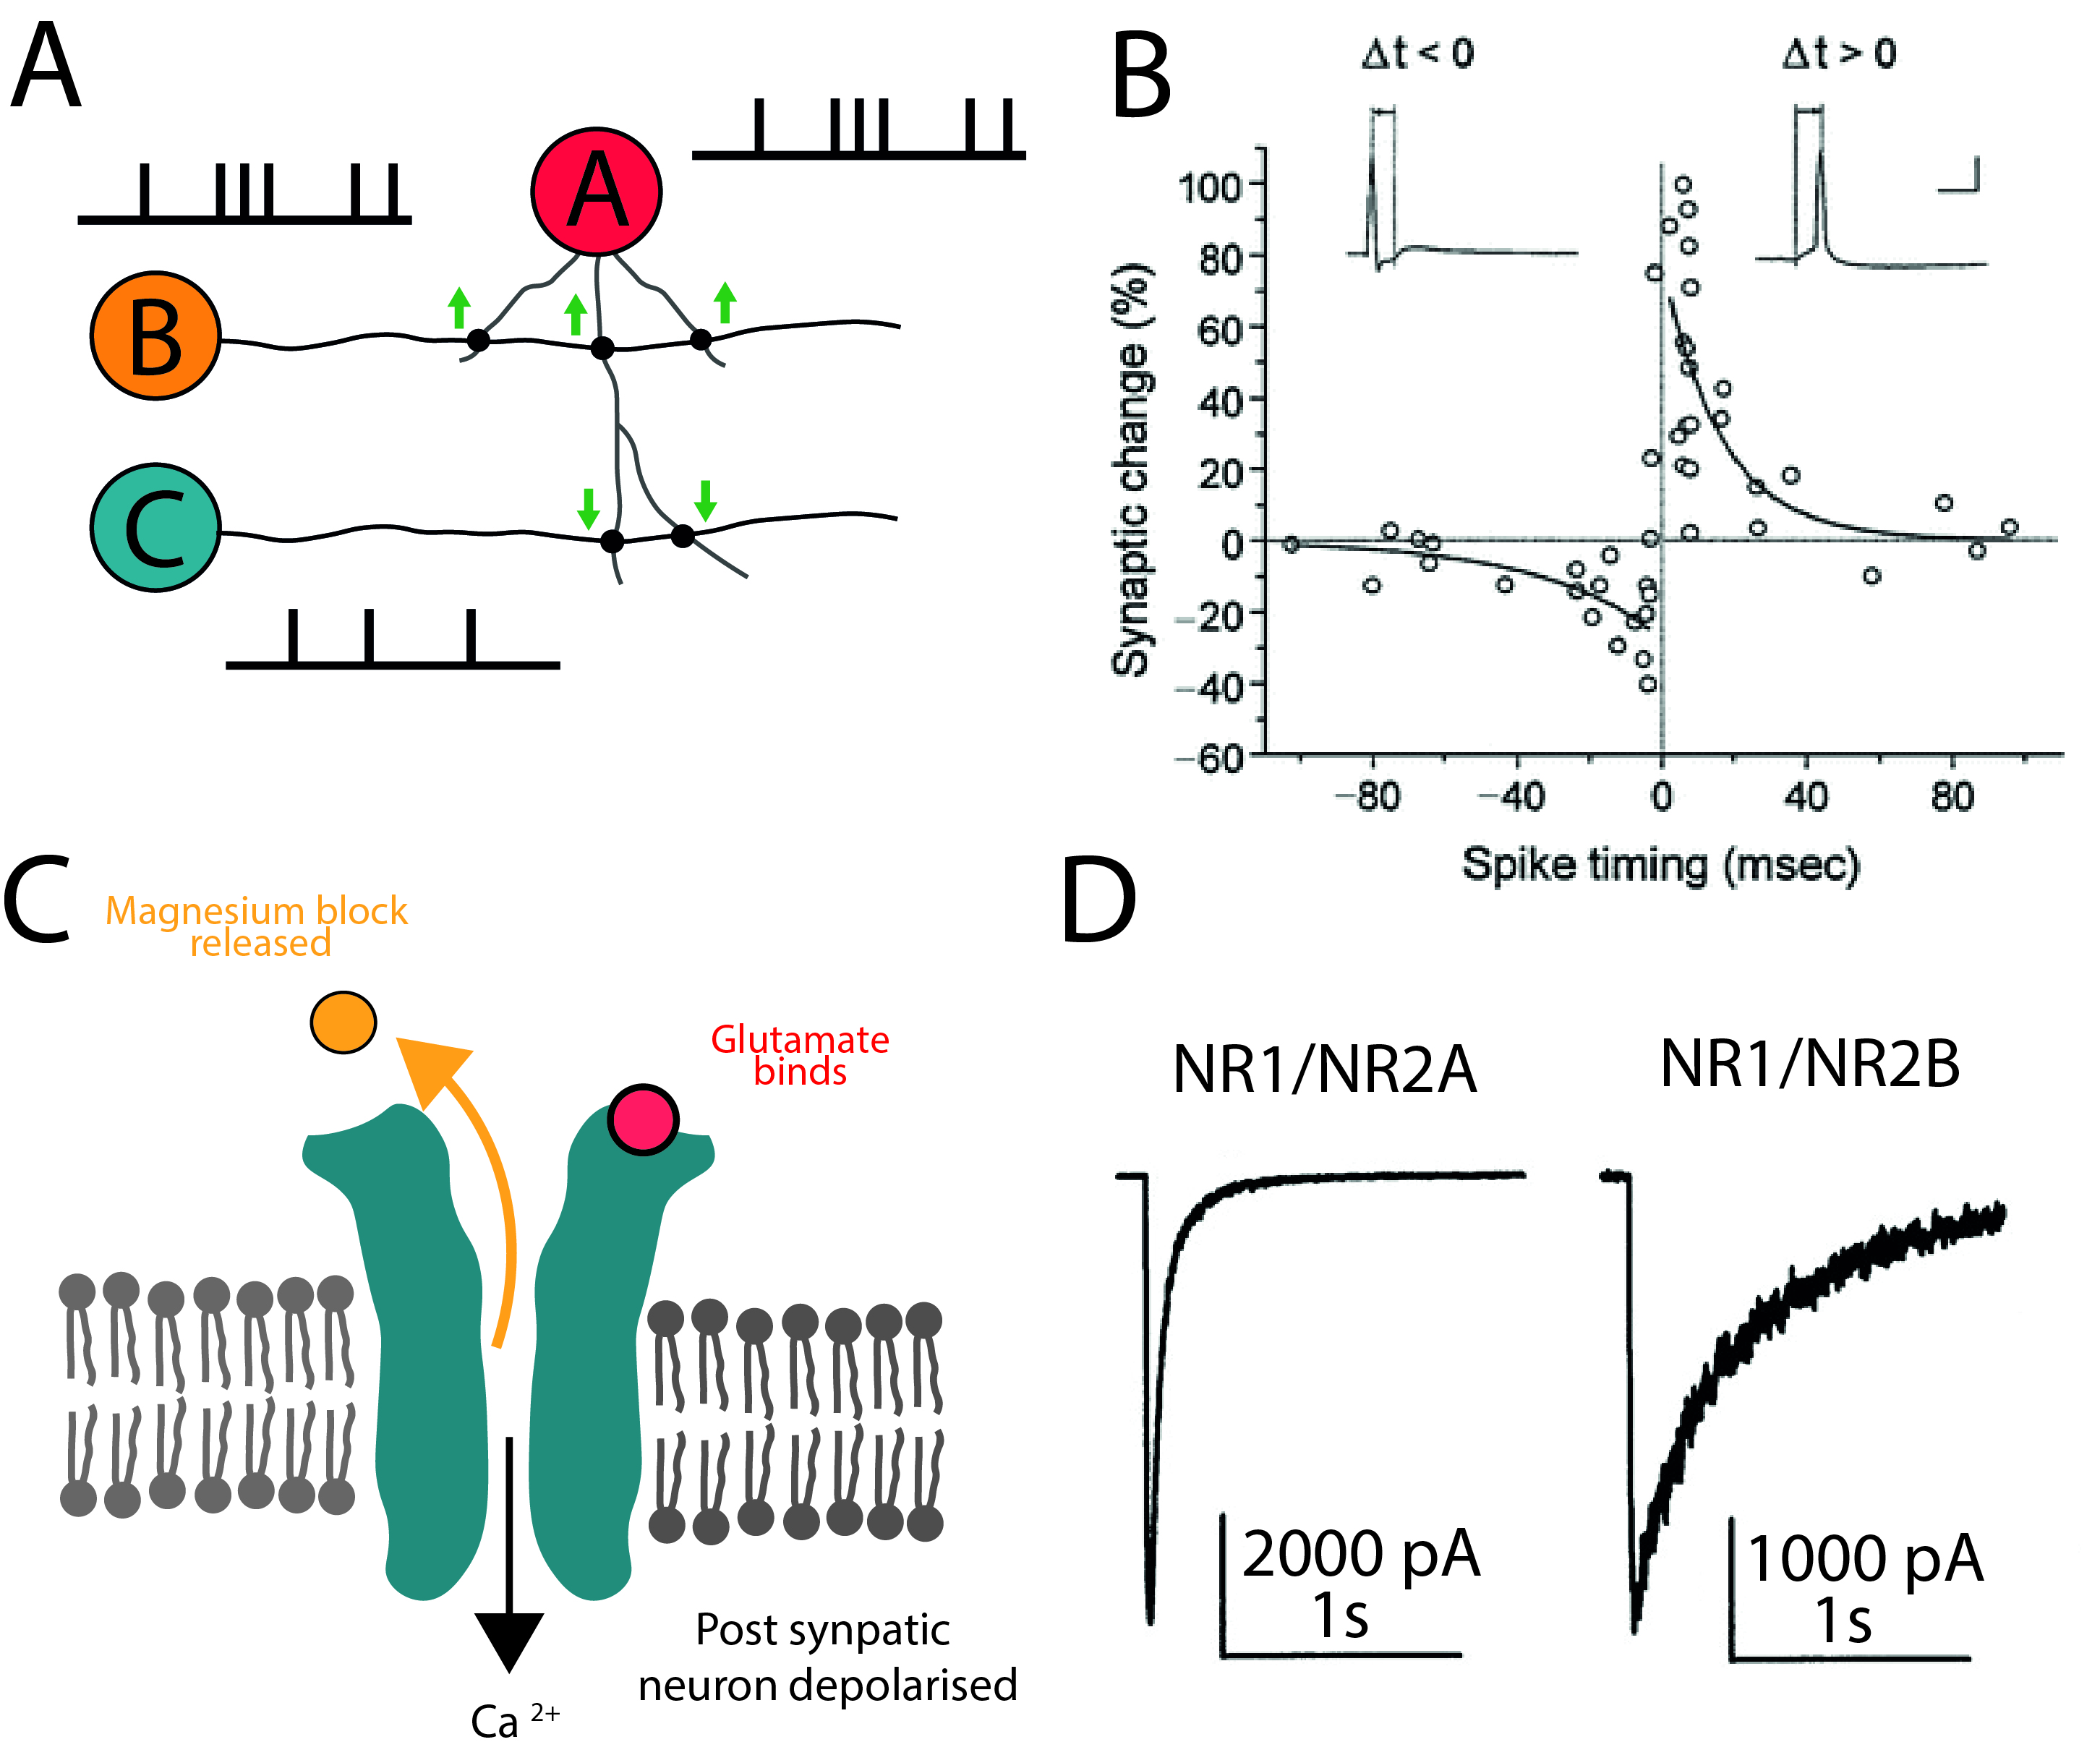
\includegraphics[width =  0.7\paperwidth]{Figures/I_hebbian_plasiticty_fig.jpg}}
            \caption[\textbf{\label{fig:I_hebbian_plasiticty_fig}\textbf{Visual experience can cause synaptic changes through Hebbian plasticity.}}]{ \textbf{\label{fig:I_hebbian_plasiticty_fig} Visual experience can cause synaptic changes through Hebbian plasticity.} \textbf{(A)} Hebb’s rule: When neurons are correlated in their firing pattern (such as neuron A and B) the synapses between them get stronger through a process of LTP. Neurons that are decorrelated in their firing patterns (neuron A and C) result in weakening of synapses through LTD. \textbf{(B)} A plot showing the change in synaptic strength when the postsynaptic neuron fires at different times relative to the presynaptic neuron ($\delta$t). Here a $\delta$t of 0 indicates that both neurons fire at the same time. When postsynaptic spikes precede the presynaptic spike ($\delta$t < 0), synapses undergo LTD whereas if they follow the presynaptic neurons ($\delta$t > 0), synapse undergo LTP. The extent of the synaptic change exponentially decays as $\delta$t moves away from 0. From (\cite{Bengio2015STDPActivity}). \textbf{(C)} The NMDAR acts as a coincidence detector between pre- and postsynaptic activity, facilitating hebbian plasticity. The pore of the channel is only open when the following two conditions are met: glutamate is bound to the receptor, and the postsynaptic cell is depolarized, removing the Mg2+ blocking the channel, this allows for Ca2+ influx. \textbf{(D)} NMDA channel kinetics depend on the receptors subunit composition. NR1/NR2A NMDAs have a fast opening probability and fast decay kinetics. NR21/NR2B NMDAs have a much slower decay and a lower opening probability. Note that the peak current of NR1/NR2A channels is much higher than NR1/NR2B channels. However, the NR2B containing channel carries around 2-fold the charge overall because of the much longer decay kinetics. Image from  (\cite{Chen1999Subtype-dependenceProbability}).

        }
      \end{figure}

\section{How does natural visual experience influence the formation of visual behaviour and population activity?}

Many of the traditional approaches to studying the effects of visual experience on the developing visual system have relied upon artificial manipulations of the visual input, such as dark rearing, strobe rearing, and stripe rearing. These manipulations have been instrumental in demonstrating that visual experience can instruct the development of the various properties of the visual system, including visual map formation, neuron morphology, and tuning properties of neurons. Furthermore, they suggest that the developing visual system, through modifications in synaptic weights, is able to encode the statistics of the visual environment.  However, the overarching role of the visual system is to drive visual behaviours. Despite this, very few studies examining experience-dependent plasticity in the brain have also looked at behaviour. This maybe due to the fact that in studies were animals have been dark reared, due to the severity of the manipulation, visuomotor behaviour was completely abolished (\cite{Kalil1978DarkNucleus, Mower1982BehavioralCat, Avitan2017}). While this shows that visual experience is required for visual behaviours to develop, it is possible that different types of experience shape behaviours in different ways, potentially even enhancing its performance. In line with this, a small number of studies have shown that visual conditioning can have powerful effects in modifying behaviour on relatively short time scales. For example, following a brief exposure to a moving grating \textit{xenopus} tadpoles have been shown to exhibit more varied levels off acceleration when swimming over counterphased gratings, suggesting that they have improved visual discrimination (\cite{Schwartz2011Activity-DependentDevelopment}). Interestingly, these behavioural changes are reflected by an increased sensitivity of direction selective neurons for the trained direction and this development requires the synthesis of the neurotropic factor BDNF. Interestingly, this same conditioning stimulus can also modify other behaviours with conditioned tadploes being far more likely to swim away from an approaching object (\cite{Shen2014AcuteXenopus}). These studies demonstrate that even a short exposure to certain visual stimuli is capable of shaping behaviour. Based on this it likely that sustained exposure to different visual stimuli through development as the visual system is being assembled could have far more dramatic effects on the ontogeny of behaviour. 

Despite this, no study to date has examined the effect of altered visual scenes during development alongside behaviour. Therefore an aim of this thesis is to do just this, by manipulating the visual scene through \gls{ee} and observe how behaviour is affected. In particular it aims to manipulate the visual scene by mimicking the statistics of visual scenes that would be observed by animals in their natural habitats. If this manipulation has an effect on behaviour, it will be imperative to understand what aspects of brain development may be underlying these effects. To do this, it is important to first consider what aspects of brain function underlie the generation of behaviour in order to look at the most relevant scale. Often due to restrictions in methodology, the effect of visual experience on the development of the visual system has typically been measured by looking at single neurons or sensory maps. However, behaviour is likely to be an emergent property of multiple neurons firing in a distributed populations (\cite{Yuste2005, Saxena2019TowardsDoctrine, Eichenbaum2017}). Therefore, if we want to understand how changes in behaviour are relate to changes in the brain it is necessary to look at developing activity in neural populations. This section introduces the idea of manipulating the visual scene through \gls{ee} and previous attempts to study the effect of visual experience on developing population activity.

\subsection{Environmental enrichment: naturalistic manipulations to the visual scene}

Firstly, traditional sensory manipulations in neuroscience can be considered as relatively extreme. This is because they do not recapitulate features contained within naturalistic visual scenes that an animal would usually be exposed to. Even for animals that are raised under normal laboratory conditions, the visual experience is likely to be highly impoverished compared to those that an animal would experience in their natural habitat. This is because natural scenes are complex, containing different spatial frequencies, colors and different types of motion. Experiences of these features are likely to produce very different correlation patterns within the retina, shaping connectivity and therefore the computations that the visual system can perform. How these naturalistic features contribute to visual system development is still relatively unknown.

Rather than limiting an animal's sensory experience, an alternative strategy is to enhance it through \gls{ee}. This is where the housing of an animal is modified to increase the amount of cognitive, motor, and sensory experience relative to “standard” rearing conditions (\cite{Nithianantharajah2006EnrichedSystem}). Typically, this has been done in rodents by rearing them in a larger cage, providing them with natural bedding, and a diverse array of novel objects to promote voluntary exploration of the environment (\cite{Alwis2014EnvironmentalInjury}). In addition to this, some studies have also raised rodents with other cage mates, providing social enrichment. Early studies of EE observed that it could induce wide ranging changes in terms of anatomy, gene expression, and behaviour (\cite{Hebb1947TheMaturity., Bennett1964ChemicalBrain, Diamond1976EffectsHippocampus}). In the visual system specifically, EE can make neurons more responsive to light, sharpen the tuning profiles of orientation selective cells, improve visual acuity, and increase contrast sensitivity (\cite{ Beaulieu1990EffectProperties, Beaulieu1990EffectCharacteristics, Mainardi2010EnvironmentalCortex}. EE has also been reported to accelerate the development of many aspects of the visual system (\cite{Cancedda2004AccelerationEnrichment}) and alter the branching patterns of neurons in the visual cortex (\cite{Greenough1973PatternEnvironments}). Furthermore, while OD plasticity in mammals is usually restricted to the critical period, exposing adult mice to enrichment for 3 weeks prior to MD reactivates high levels of plasticity in cortical granule cells (\cite{Baroncelli2010Experience-dependentCortex}). This reawakens OD plasticity in the visual cortex, resulting in depressed visually evoked activity when the deprived eye is stimulated, suggesting that EE can regulate how plastic cortical neurons are. 

Despite this wide range of effects on the visual system, typical EE protocols are often multisensory, making it difficult to understand whether these changes are the result of altered visual experience, experience across other modalities, increased motor activity through exploratory behavior, or a combination of all of these. While some modality-specific enrichments have been performed in the auditory system, currently no study has provided a manipulation that specifically enriches visual experience. Such manipulations, using naturalistic visual stimuli will be crucial for understanding how  natural visual features shape visually guided behavior through experience-dependent changes in the brain.

\subsection{Moving from neurons and maps to population activity}

Secondly, traditional investigations of how visual experience shapes the brain during development have been limited by methodology to studying individual neurons or coarse anatomy in the form of sensory maps. A limitation of this is that for many of these recorded features, it is not known if, or how, they relate to perception and behaviour. For example, retinotopic maps were once thought to be important for encoding the position of stimuli in visual space. However, the location of responding neurons within the retinotopic map of the zebrafish tectum has been shown to be a poor predictor of stimulus position (\cite{Avitan2016}). Importantly, this predictive power of stimulus position is well below what would be required for generating the precision seen in certain visually-guided behaviours. Therefore, it is possible that retinotopy, like lamination, may be a structural feature that speeds development of the visual system rather than being an important feature for generating computations (\cite{Nikolaou2015LaminationCircuits}). Likewise, recording the activity of individual neurons during stimulus presentations or behavior has shown that their responses are extremely unreliable and noisy, limiting the information that a single neuron can encode (\cite{Avitan2016}; \cite{Graf2011DecodingCortex}). Even many simple behaviours, such as controlling the movement of the eye or arm, are far too complex  to be encoded by individual neurons (\cite{Lee1988PopulationColliculus, Lee1988PopulationColliculus,Georgopoulos1995, Averbeck2006NeuralComputation}). Instead, many of these properties are encoded through large numbers of neurons acting together in concert creating distributed population codes (\cite{Yuste2015, Saxena2019TowardsDoctrine, Buzsaki2010}). Experience-dependent changes in both sensory maps and individual neurons are indicative of, albeit from different spatial scales, changes in neural circuitry. These changes are likely to manifest as changes in the organization of population activity. Therefore if we want to relate visually dependent changes in the brain to changes in behaviour it is necessary to describe how population activity is shaped by the visual scene.

In the last decade, there have been drastic advancements in recording techniques that allow for the neural activity from thousands of neurons to be recorded simultaneously (\cite{Broussard2014MonitoringIndicators, Jun2017FullyActivity,Nicolelis2003ChronicMonkeys}). One  of these developments is that of calcium imaging.  Calcium indicators are proteins that report changes in calcium concentration through changes in fluorescence intensity,  allowing them to act as indicators of neural activity as calcium floods into a cell during an action potential (\cite{Akerboom2013GeneticallyOptogenetics}). These indicators can either be genetically encoded or injected as dyes, allowing large numbers of neurons to be labeled (\cite{Dunfield2010InBrain., Tian2012ImagingIndicators}). Imaging the resulting fluorescence changes with fast imaging methods allows for the neural activity of thousands of neurons to be monitored with single neuron resolution (\cite{Ahrens2013, Sofroniew2016AImaging}). Alternatively, multisite electrode shanks can be inserted into the brain, with minimal damage, allowing for the activity of multiple neurons to be recorded with high temporal resolution (\cite{Jun2017FullyActivity, Nicolelis2003ChronicMonkeys}). Such recording techniques allow the effects of visual experience on the development of the organisation of population activity to be examined in the brains of awake animals.

A feature of population activity is synchronous activations of groups of neurons, known as neural assemblies (or ensembles) (\cite{Buzsaki2010, Yuste2015}). Such assemblies have been found to be activated by certain stimuli and are more predictive of behavioural states than single neurons (\cite{Miller2014, Carrillo-Reid2015, Stringer2019SpontaneousActivity,Deolindo2018NeuronalRats, Diana2019BayesianAssemblies}).  As a result, it has been proposed that the synchronous activity of multiple neurons could collectively build emergent properties that are not present in at the level of the single neuron constituents, acting as the functional units of the brain (\cite{Hopfield1982,Yuste2011,Yuste2015,Saxena2019TowardsDoctrine}). Synchrony in the mammalian cortex can preferentially occur between neurons that share similar tuning properties (feature-selective synchrony) (\cite{Gray1989,Denman2014TheMap., Ishikawa2018Experience-dependentCortex}) This feature-selective synchrony is thought to be important for efficiently driving downstream target neurons, allowing for robust signal transmission (\cite{Usrey1999SYNCHRONOUSSYSTEM,Bruno2006CortexSynapses, Ishikawa2018Experience-dependentCortex}). In mice, there is increased connectivity between pyramidal neurons in the cortex neurons with the same orientation selectivity (\cite{Ko2011}). These connections develop shortly after eye opening and correlate with the onset of feature-selective synchrony (\cite{Ko2013, Ishikawa2018Experience-dependentCortex}). This suggests that the development of synchrony in the cortex may be driven by visual experience. Dark rearing or binocular deprivation through eye suturing blocks the development of feature-selective synchrony, showing that visual experience is integral for establishing feature-selective synchrony (\cite{Ishikawa2018Experience-dependentCortex}).  Recently, a study showed that in principle synchronous activity in the cortex could be established through Hebbian mechanisms (\cite{Carrillo-Reid2016}). In this study, calcium indicators were expressed in cortical neurons alongside a light sensitive ion channel, channelrhodopsin. The expression of this protein enabled photoactivation of multiple neurons simultaneously by targeting them with a two-photon laser, through a process known as optogenetic stimulation. Some neighbouring neurons initially had low levels of correlated activity with each other. However,  repeatedly photo-stimulating these neurons resulted in them spontaneously firing in synchrony with each other, effectively imprinting an artificial neural assembly within the brain. Therefore it is possible that during development neurons could be bound together in an assembly based on the fact that they are responding to the same visual feature in the environment.

The accessibility of the optic tectum of tadpoles allows for the spatiotemporal structure of developing population activity to be studied using calcium imaging. In the tectum correlated activity can result from either tectal neurons being activated by the same visual stimulus via RGCs or from intertectal recurrent connectivity (\cite{Pratt2008DevelopmentTectum}). In \textit{xenopus} activating RGCs with a whole field light stimulus demonstrated that the degree of correlations between tectal neurons increased between developmental stages 44 and 49, and the responses of neurons became more reliable between trials. These correlations are likely to reflect changes in local circuitry because similar increases in correlation are seen in spontaneous activity in isolated brain preparations where the retina is absent. This development of correlated activity depends on visual experience because dark rearing eliminates it (\cite{Xu2011VisualSystem}). This suggests that feedforward visual experience shapes local tectal circuitry, leading to more robust responses to visual stimuli. Furthermore, the spatial structure of correlations between neurons in the tectum can be shaped through visual training by repeated exposure (2 hr) to stimuli moving in different directions (\cite{Podgorski2012}). This leads to high levels of local correlations between neighbouring neurons, which become tuned to similar orientations. In contrast, neurons that are further away from each other are tuned to different orientations and their correlations decrease. Importantly, through training the ability to decode the stimulus identity from the population activity also increased. This indicates that these plastic changes may be important for improving the sensory representation of previously experienced visual stimuli.

One approach that has proven to be particularly useful in studying developing population activity in zebrafish is to record spontaneous activity from the optic tectum when the larvae are in total darkness (\cite{Romano2015, Avitan2017, Pietri2017}). This is because spontaneous activity is not simply random. Instead correlated activity is likely to occur between neurons that are connected (\cite{Marachlian2018PrinciplesTectum}), rather than being driven by a common source from the retina. Supporting this correlated activity between neurons in the tectum persists following eye removal at 7 dpf, suggesting that this activity is driven by local circuits (\cite{Romano2015}). This correlated activity is caused by spatially compact neural assemblies. Importantly, these spontaneously active tectal assemblies resemble those that are activated by prey-like stimuli or tail movements (\cite{Romano2015}). This suggests that studying spontaneous activity acts as a proxy for functional connectivity within the tectum (\cite{Marachlian2018PrinciplesTectum}). 
The development of tectal population activity relies on input from the retina because removing the eye increases the amplitude, frequency and synchronisation of calcium events in tectal neurons (\cite{Pietri2017}). While the number and spatial extent of neural assemblies were slightly reduced, they were still found throughout the tectum, suggesting their development is partially intrinsically driven. In addition to eye removal, Avitian et al.,  (\citeyear{Avitan2017}) also looked at the effect of dark rearing on both tectal spontaneous activity and behaviour. They found that dark reared fish had substantial changes in population activity with reduced pairwise correlation between neurons, reduced assembly number and reduced functional connectivity within assembly. Alongside this, the hunting performance of dark reared fish was severely reduced compared to normally reared fish. This is significant because single neuron activity and tuning properties in this study and others were unaffected by dark rearing (\cite{Avitan2017}; \cite{Niell2005FunctionalTectum}). This suggests that it is circuit level changes in population activity that may underlie the changes in behavioural performance. 

Together these studies demonstrate that visual experience is necessary to shape certain aspects of developing population activity and visually guided behaviours such as prey capture. However, currently no study has attempted to look at how these aspects of brain development are affected by different types of visual experience, such as naturalistic visual features. Such features may be important for shaping certain aspects of the visual system and may even enhance behavioural performance relative to normal lab conditions. Therefore the aim of this thesis is to examine how behaviour and developing population activity are modified through exposure to naturalistic features in an EE. In addition, it aims to understand how the subunit composition of the NMDAR facilitates these experience-dependent changes. As evidenced by many of the studies cited in this chapter, the larval zebrafish has often been used to study experience-dependent changes. The following section will discuss the properties of this system that make it a powerful organism for studying behaviour and neural circuitry within the developing brain.

\section{Zebrafish: An ideal system to study the development of behaviour and population activity.}

\subsection{Rapid external development}
 In contrast to mammalian embryos, zebrafish larvae develop extremely rapidly. In just 7 days, zebrafish larvae transform from a single cell into a recognisable fish, capable of generating a rich repertoire of visually-guided swimming behaviours (\cite{Orger2017ZebrafishChallenges}) (\textbf{Figure \ref{fig:I_ZF}A}). This means that within this very short temporal window, all the neural circuitry required to direct those behaviours needs to be established.

Unlike amniotic species, which develop either in a thick shell or \textit{in utero}, fertilized zebrafish embryos develop externally (\cite{Pratt2016AnDevelopment}). This exposes the retina to the visual environment throughout visual system development, creating visually evoked patterns of correlated activity within RGCs as soon as the first synapses begin to form. These patterns are subsequently propagated throughout the visual system as these developing axons make their first synapses with the retinorecipient regions of the brain between 2.5-3 dpf (\cite{Niell2005FunctionalTectum}). Therefore, continual visually evoked activity has the potential to shape the development of the visual system, as visually evoked behaviour is emerging (\cite{Easter1996TheRerio, Orger2017ZebrafishChallenges}). This is perhaps important given that zebrafish habitats in the wild are known to be extremely diverse in terms of the visual features they contain (\cite{Engeszer2007ZebrafishField}).  Experience-dependent plasticity in the face of such diversity could provide a mechanism by which genetically similar fish learn the statistics of the visual environment within which they are raised. This could potentially lead to adaptive behaviour, allowing the fish to cope with, or exploit features of the environment. Furthermore, due to their external development the effect of the visual environment on brain development can be studied by simply manipulating the statistics of the visual scene that surrounds a petri dish of embryos. This allows for purely visual EE to be performed using naturalistic stimuli.

\subsection{Quantitative analysis of visually guided behaviour}

Even as visual circuits are developing, zebrafish rely heavily on incoming visual information for survival, producing a wide repertoire of visually-guided behaviours. These behaviours can be readily studied in the laboratory using high-speed cameras and custom built trackers (\cite{Orger2017ZebrafishChallenges}). These trackers allow for simultaneous estimation of heading direction, eye angle, and tail position, allowing the kinematics of behaviour to be accurately quantified. 

From just 3 dpf zebrafish start to show viusally driven behavioural responses to visual stimuli (\cite{Easter1996TheRerio}). This coincides with the first RGC input reaching the retinorecipient regions of the brain (\cite{Burrill1994DevelopmentRerio, Easter1997TheRerio}). These include reflexive movements of the eyes in response to rotational motion (OKR) and the \gls{omr}, where the larvae swim in the direction of whole field motion so that they can stabilize their position with respect to their environment (\cite{Naumann2016FromResponse, Portugues2015Whole-fieldProcess, Kubo2014}). Additionally, zebrafish perform high velocity "c-turn" escape behaviours to avoid being eaten by predators or colliding with objects (\cite{Dunn2016}).   However, perhaps the most intricate and complex of these early visual behaviours is that of prey capture (\cite{Budick2000LocomotorCapture}). For zebrafish, prey are small motile organisms, such as rotifers or paramecia. Zebrafish hunt and consume these prey in a well-described sequence of movements, providing them with the nutritional content needed for them to survive (\cite{Budick2000LocomotorCapture, Gahtan2005, Patterson2013, McElligott2005PreyControl} (\textbf{Figure \ref{fig:I_ZF}B-C}). First, larvae must distinguish a potential target from the rest of the visual scene, locate its position in visual space, and decide whether or not it is worth eating. If hunting is initiated, larvae converge their eyes and orientate themselves towards the prey using characteristic J-turns, unilateral bends of the tail-tip in the direction of the prey. Correctly orientated larvae then perform a series of forward swims approaching the prey, catching it with a final consummatory high-velocity strike. In addition to freely swimming fish, prey capture can be elicited in head fixed larvae using artificial stimuli presented on a screen. In these setups, eye convergence and J-turns can be induced by prey-like stimuli - small moving dots between 1 and 10 degrees  (\cite{Bianco2015, Semmelhack2014, Bianco2011, Jouary2016ALarvae}). 

Prey capture is often considered to be an innate behaviour which emerges around 5 dpf and improves towards 7 dpf. Although this improvement could be the result of developmental changes in the hydrodynamics of the fish, a recent study showed that these changes in hunting performance correlated with a refinement of the neural representation of the location of prey-like stimuli within the tectum  (\cite{Avitan2019}). It is possible that this refinement reflects the continued organisation of neural circuitry driven by intrinsic factors. However, prior exposure of larvae to live prey modifies the aspects of the behavioural sequence leading to more efficient captures (\cite{Lagogiannis2019LearningLarvae}). This indicates that there are aspects of hunting that are learnt through experience. Therefore, studying prey capture gives an opportunity to understand how manipulations to the visual environment may affect a naturalistic visually guided behaviour within a laboratory setting.

\subsection{The zebrafish optic tectum}
The optic tectum of zebrafish is known to be an important central hub for processing sensory information (\cite{Nevin2010}). It uses this information to generate visually guided behaviour such as approach maneuvers towards a prey or predator avoidance. As such, tectal ablations abolish these behaviours (\cite{Gahtan2005}) but leave other visuomotor behaviour intact (\cite{Roeser2003}). The optic tectum can be divided into two main regions: a deep region containing the cell bodies of tectal neurons, known as the stratum pervienticular (SPV) layer, and a more superficial region consisting of dense neuropil (\textbf{Figure \ref{fig:I_ZF}D}). Afferent projections to the tectum come from different sensory modalities. These projections target the tectum via the neuropil region and terminate within specific laminae (\cite{Xiao2005AProjection, Xiao2007Lamina-specificDragnet}). The most significant of these afferent projections comes from the retina.  Incoming RGCs terminate in the superficial lamina in a retinotopic fashion whereas other sensory modalities innervate laminae deeper within the neuropil. The retinal input to the optic tectum has been found to be highly organised with different direction selective RGCs targeting distinct sublaminae, with each one containing its own retinotopic map (\cite{Nikolaou2012ParametricTectum, Xiao2007Lamina-specificDragnet}). 

Downstream of the tectal afferents are tectal neurons which extend their dendrites into the tectal neuropil, sampling from the incomming sensory input (\cite{Kinoshita2006RolesTectum}). Tectal neurons have been found to have diverse morphologies and many neurons have axons that terminate within the same tectal hemisphere whereas others terminate contralaterally (\cite{Scott2007TargetingTrapping, Scott2009TheLines, Gebhardt2019AnTectum}). This suggests that like the tectum of frogs (\cite{Pratt2008DevelopmentTectum}), zebrafish may possess a high degree of recurrent connectivity which processes and integrates sensory input. Tectal neurons are known to be tuned to a range of different visual features such as size (\cite{DelBene2010FilteringCircuit}), direction (\cite{Hunter2013, Grama2012DirectionInhibition}) and orientation (\cite{Hunter2013}).  These neurons are grouped together into spatially compact neural assemblies which are thought to contain neurons with different tuning properties (\cite{Romano2015, Bianco2015, Dunn2016}). Tectal assemblies can be activated by ethologically relevant stimuli such as those that resemble prey or predators  (\cite{Bianco2015, Romano2015, Dunn2016, Avitan2019}). Furthermore, these assemblies are more predictive of hunting and escape behaviours than tectal neurons, suggesting that they act as population codes driving these visuomotor behaviours (\cite{Avitan2016, Avitan2019, Dunn2016})

In addition to a retinotopic map of visual space, the tectum also contains a map of motor actions. This is because stimulating different regions along the anterior-posterior axis of the tectum, generates different behaviours. (\cite{Herrero1998TailGoldfish}; \cite{Helmbrecht2018}; \cite{Fajardo2013ControlZebrafish.}). For example, high angle tail bends that resemble C-turn escape maneuvers can be elicited with a higher probability through stimulation of the posterior regions of tectum. J-turns, on the other hand, show less of a spatial bias but higher angle tail bends are elicited when the stimulation site is more posterior (\cite{Helmbrecht2018}). The tectum drives these movements through the many tectal efferent projections which target various motor centers in the mid- and hindbrain  (\cite{Helmbrecht2018}) (\textbf{Figure \ref{fig:I_ZF}E}). 

\subsection{Large scale population imaging}
Zebrafish are highly genetically tractable, allowing for genetically encoded calcium indicators to be expressed under pan-neuronal promoters (\cite{Kim2014ProlongedMapping}) (\textbf{Figure \ref{fig:I_ZF}F}). Furthermore, due to their small size and optical transparency the optic tectum, and even the whole brain, can fit comfortably in the field of view of a single microscope objective. This allows for the neural activity of thousands of neurons to be sampled multiple times a second, with single neuron resolution (\cite{Ahrens2013,Bianco2015,Portugues2014}). These experiments can be combined with virtual reality setups where fish are presented with visual stimuli whilst their tail movements are simultaneously recorded (\cite{Bianco2015, Semmelhack2014, Naumann2016FromResponse, Portugues2014}). Such techniques have proven to be extremely useful for dissecting the neural circuitry underlying visually-driven behaviours. Alternatively, spontaneous activity can be recorded to understand how functional connectivity in the tectum is altered either by developmental stage or manipulation (\cite{Avitan2017, Pietri2017}). Therefore, recording either spontaneous or visually evoked activity can be used to understand how aspects of population activity in the developing visual system is shaped by the visual scene. As a result, these properties of the larval zebrafish make it an ideal system for interrogating the effects of the EE on the development of both prey capture and underlying population activity within the optic tectum. 

\clearpage
\begin{figure}[]
        \center{\includegraphics[width =  0.67\paperwidth]{Figures/I_Zebrafish_intro_v2.jpg}}
            \caption[\textbf{\label{fig:I_ZF}\textbf{Zebrafish as a model organism to study the effect of EE on visual behaviour and population activity in the tectum. }}]{ \textbf{\label{fig:I_ZF} zebrafish as a model organism to study the effect of EE on visual behaviour and population activity in the tectum.} \textbf{(A)} Zebrafish have a rapid external development. They go from a single cell (0 hours post fertilization - hpf) to a recognisable fish that is capable of generating visually driven behaviours in 5 days. \textbf{(B)} Frames from a movie of a zebrafish hunting down its prey (in this case a paramecium) which is marked by the orange arrow tip. Images from (\cite{Bianco2011}) \textbf{(C)} Schematic illustrating that during prey capture larval zebrafish converge their eyes and make “J-turns”. These turns, through a unilateral bend of the tail tip, orientate the fish towards the prey. Such movements are characteristic of prey capture, allowing for it to be distinguished from other behaviours. \textbf{(D)}  Schematic of tectal organisation to illustrate that incoming RGCs from the contralateral eye terminate in the tectal neuropil (NP). PVN cells (blue), with their cell body in the SPV extend their dendrites into the NP where they receive incoming sensory input. Many PVN neurons are organised into tectal assemblies (represented by the groups of neurons in green and yellow), which have been found to be active spontaneously and under visually evoked conditions. \textbf{(E)} A map of tectal efferents with both dorsal (left) and lateral views (right). Efferents are colored according to their projection class (bottom right table). Tectal effects project to multiple different motor targets in the tegmental midbrain and hindbrain (tectobulbar projections) in both ipsi- and contralateral projections. These are thought to be important for directing visually driven behaviours. Image from (\cite{Helmbrecht2018}). \textbf{(F)} A widefield image of a head fixed zebrafish expressing a calcium indicator in its optic tectum. The arrow points to a paramecium which is seen by the left eye causing a corresponding activation of tectal neurons in the contralateral tectal hemisphere. Image from (\cite{Muto2013PreyFunctions}).


        }
      \end{figure}

\clearpage

\subsection{Thesis Aims}
This thesis aims to understand how visual experience, in the form of naturalistic EE, influences the development of the visual system by using the larval zebrafish as a model organism.  The main biological questions to be addressed are: How does EE shape visually driven behaviour? Does EE shape developing tectal activity? and if so, what aspects of plasticity are important for these changes to occur? Finally, and perhaps most importantly, how do changes in tectal population activity development relate to changes in behaviour? These questions have been addressed through the following three results chapters:

\begin{enumerate}
    \item Prior to answering these questions it is important to be able to reliably describe the structure and dynamics of developing population activity. Therefore a recently developed bayesian inference method was applied to spontaneous activity in the tectum to give probabilistic estimates of neural assembly number, membership and dynamics (\textbf{Chapter 3}).
    
    \item To understand the effect of EE on visual system development zebrafish were raised in enriched environments (over a bed of gravel) or under normal laboratory conditions. The effect of this manipulation on behaviour was studied by examining how the prey consumption differed between these two rearing conditions. Following this, the development of spontaneously active neural assemblies was monitored to understand both how tectal functional connectivity was impacted by the visual environment and at what point in development these changes occurred. To examine the role of Hebbian plasticity and NMDAR subunit composition in facilitating experience-dependent effects in the tectum the effect of EE was studied in a novel zebrafish mutant. This mutant was a double KO of both paralogs of the genes encoding the NR2A receptor (\textit{grin2aa} and \textit{grin2ab}), a subunit that is known to shape plasticity in the mammalian brain (\textbf{Chapter 4}).
    
    \item Finally, to relate changes in population activity to hunting performance a “virtual reality” hunting assay was developed. This experiment setup allows for the visually evoked neural activity in the tectum to be monitored alongside tail movements while prey-like stimuli are presented. Decoding the position of these prey-like stimuli from tectal activity allows for the sensory representation of stimulus location to be investigated (\textbf{Chapter 5}). This provides an experimental setup that will be important for relating the effects of EE on the development of the tectum to changes in behaviour in future experiments. 
    
\end{enumerate}
